\documentclass[aspectratio=169]{beamer}
\usepackage{hyperref}
\usepackage[T1]{fontenc}
\usepackage[spanish]{babel}
\usepackage{csquotes}
\usepackage{tribhuvan}

\usepackage{latexsym,amsmath,xcolor,multicol,booktabs,calligra}
\usepackage{graphicx,pstricks,listings,stackengine}

\author{Rodrigo Pérez Rodríguez}
\title{Tecnologías Robóticas para la Discapacidad Intelectual}
\subtitle{Percepción: láser, imagen, deep learning y razonamiento espacial}
\date{}
\setbeamertemplate{date}{}

\AtBeginSection[]{
  \begin{frame}[plain]
    \vfill
    \begin{center}
      {\LARGE\bfseries \insertsectionhead}
    \end{center}
    \vfill
  \end{frame}
}
\AtBeginSubsection[]{}

\def\cmd#1{\texttt{\color{red}\footnotesize $\backslash$#1}}
\def\env#1{\texttt{\color{blue}\footnotesize #1}}
\definecolor{deepblue}{rgb}{0,0,0.5}
\definecolor{deepred}{rgb}{0.6,0,0}
\definecolor{deepgreen}{rgb}{0,0.5,0}
\definecolor{halfgray}{gray}{0.55}

\lstset{
    basicstyle=\ttfamily\small,
    keywordstyle=\bfseries\color{deepblue},
    emphstyle=\ttfamily\color{deepred},
    stringstyle=\color{deepgreen},
    numbers=left,
    numberstyle=\small\color{halfgray},
    rulesepcolor=\color{red!20!green!20!blue!20},
    frame=shadowbox,
}

\begin{document}

\begin{frame}
    \titlepage
\end{frame}

\begin{frame}
    \tableofcontents[sectionstyle=show,subsectionstyle=show/shaded/hide,subsubsectionstyle=show/shaded/hide]
\end{frame}

\section{Percepción: láser e imagen}

\begin{frame}{De sensor a percepción útil}
  \small
  \begin{itemize}
    \item Un sensor entrega medidas crudas; percibir es transformarlas en información accionable.
    \item Pipeline típico en robótica:
    \begin{itemize}
      \item adquisición de datos,
      \item filtrado y preprocesado,
      \item extracción de características,
      \item interpretación para decisión o control.
    \end{itemize}
    \item La calidad del resultado depende tanto del sensor como del procesamiento posterior.
  \end{itemize}
\end{frame}

\begin{frame}{Marcos de referencia y transformaciones}
  \small
  \begin{itemize}
    \item Un mismo punto tiene coordenadas distintas según el marco de referencia.
    \item En ROS 2, el sistema TF mantiene la relación entre marcos en el tiempo.
    \item Idea clave: convertir todo a un marco común antes de fusionar o decidir.
    \item Composición de transformaciones:
  \end{itemize}
  \[
    T_{C \leftarrow A}=T_{C \leftarrow B} \cdot T_{B \leftarrow A}
  \]
\end{frame}

\begin{frame}{Coherencia espacio-temporal en percepción}
  \small
  \begin{itemize}
    \item La fusión sensorial requiere coherencia \textbf{espacial} y \textbf{temporal}.
    \item Sensores distintos tienen latencias y frecuencias distintas.
    \item Estrategias habituales:
    \begin{itemize}
      \item sincronización por marcas de tiempo,
      \item interpolación temporal,
      \item descarte de medidas fuera de ventana.
    \end{itemize}
    \item Sin esta coherencia, la navegación y el seguimiento de objetivos se vuelven inestables.
  \end{itemize}
\end{frame}

\section{VFF}

\begin{frame}{Virtual Force Fields}
  \small
  \begin{itemize}
    \item Simulación de fuerzas que actúan sobre un robot (como si estuviera en un campo de fuerzas real)
    \item Fuerzas:
    \item Atractiva $\rightarrow$ atrae al robot hacia su objetivo
    \item Repulsiva $\rightarrow$ empuja al robot lejos de los obstáculos
    \item Cálculos:
    \item Función de la distancia del robot al objetivo/obstáculo
    \item Suma de vectores
    \item El robot se mueve en dirección de la fuerza resultante
  \end{itemize}
\end{frame}

\begin{frame}{Ejercicio práctico}
  \small
  \begin{columns}[T,onlytextwidth]
    \begin{column}{0.58\textwidth}
      \begin{itemize}
        \item Desarrollar un nodo que haga que el robot siga una pelota por color y evite obstáculos
        \item La pelota se detectará a partir de la imagen de la cámara
        \item Los obstáculos se detectan utilizando la información del láser (el más cercano)
        \item Si la pelota no está en la imagen, el robot deberá girar hasta encontrarla
        \item Usaremos el algoritmo VFF
      \end{itemize}
    \end{column}
    \begin{column}{0.42\textwidth}
    \centering
    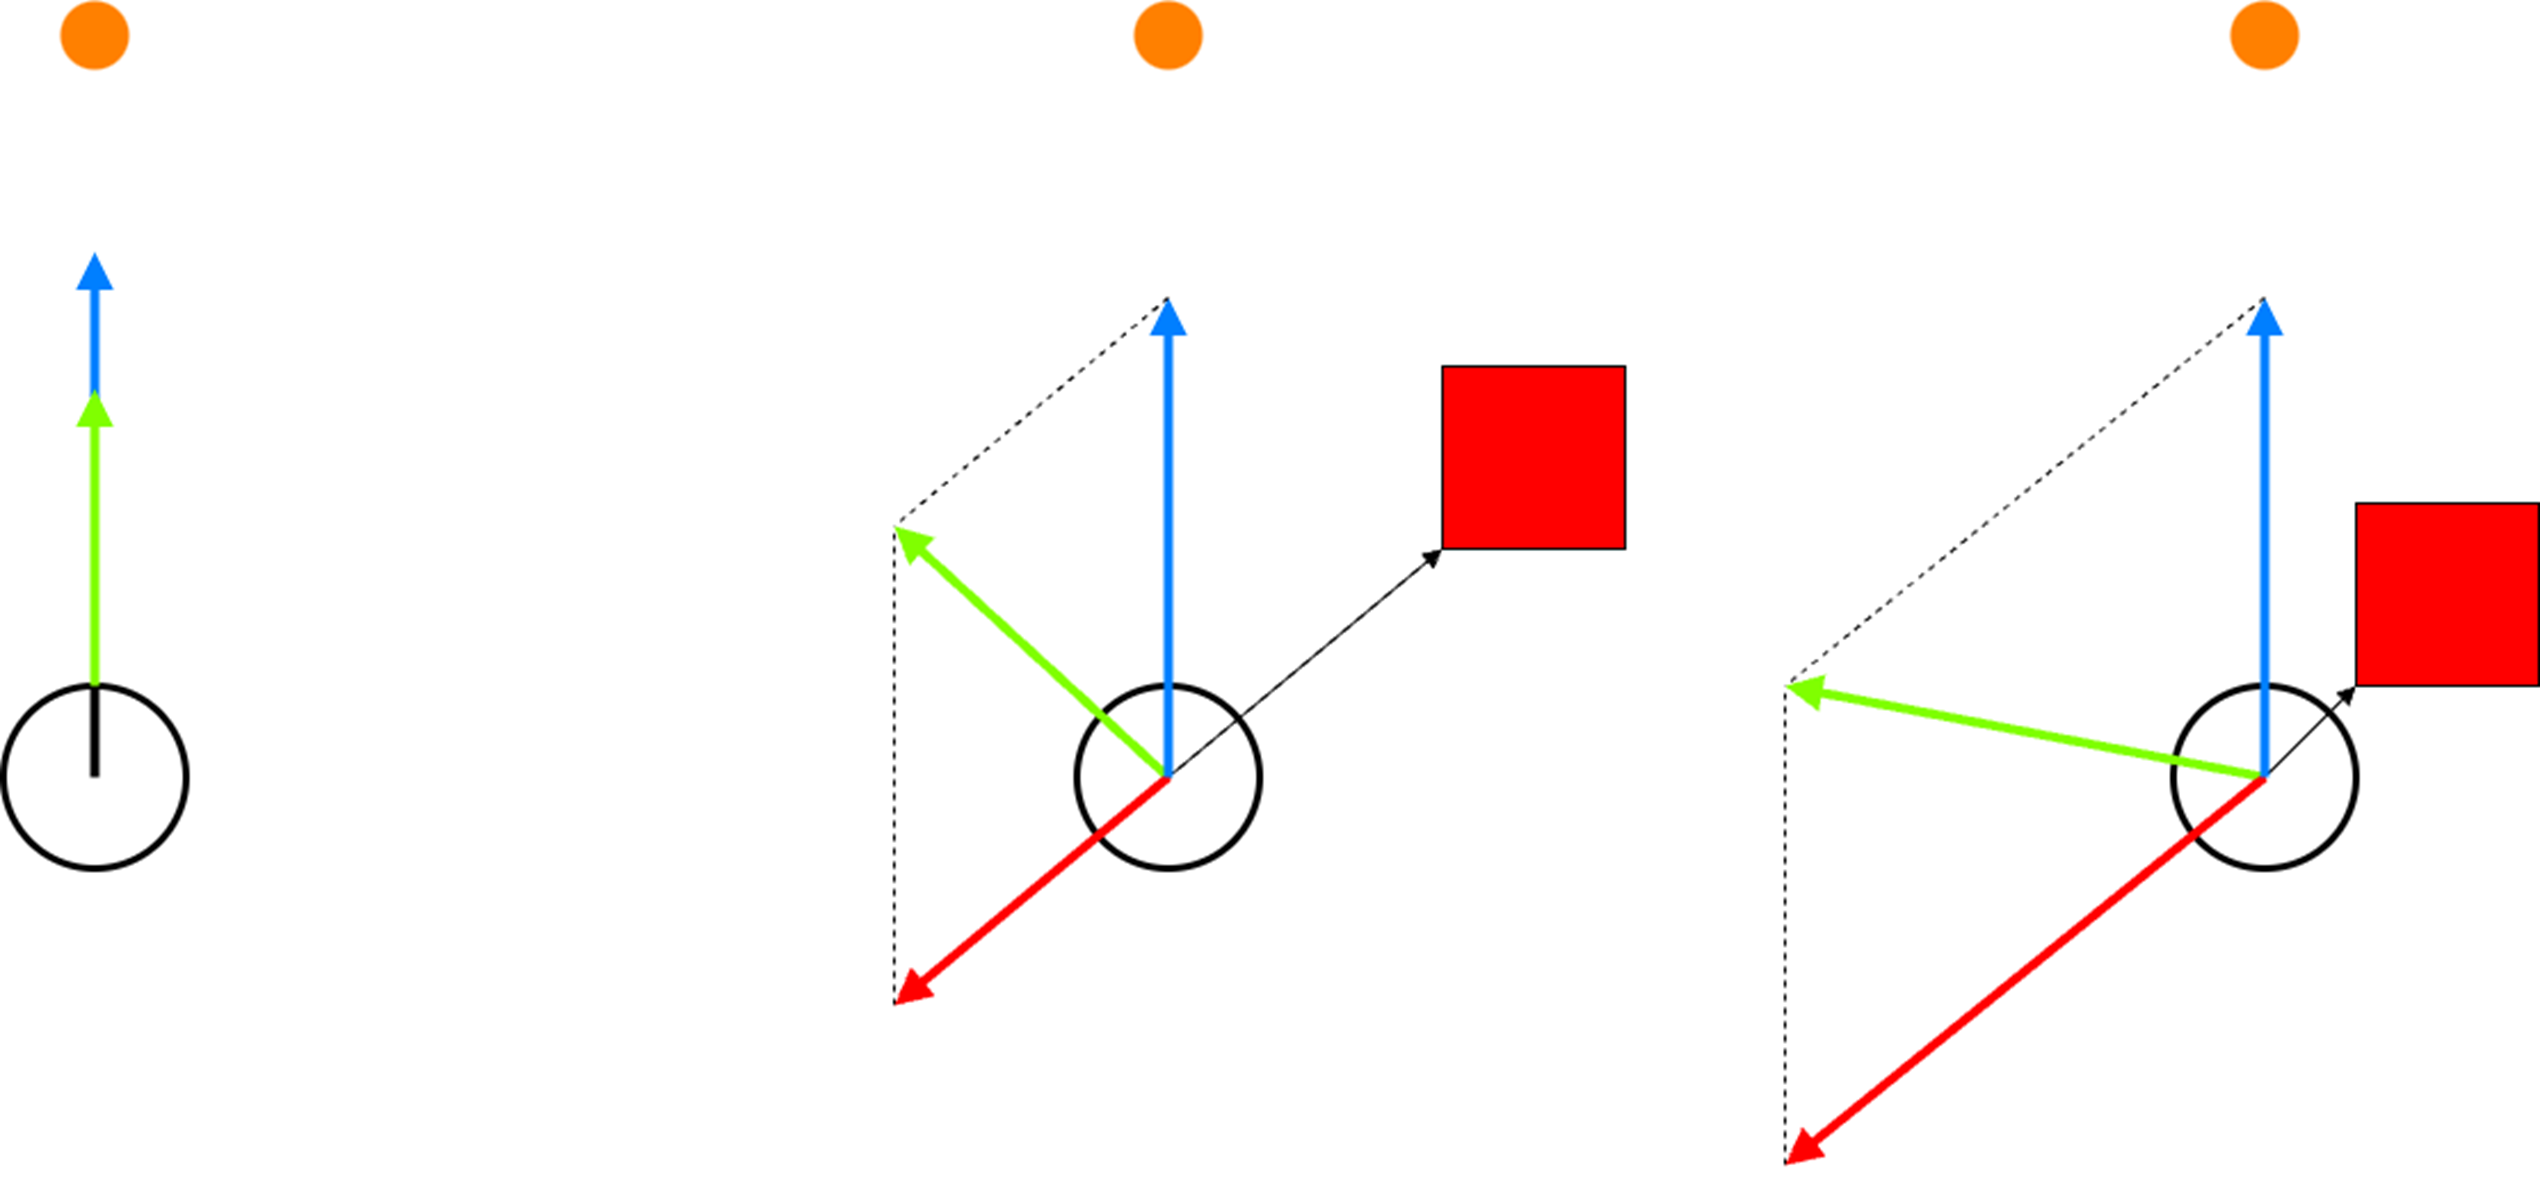
\includegraphics[width=0.95\linewidth,height=0.58\textheight,keepaspectratio]{images/tema_3/4_1_s04_ejercicio-practico_img01.png}
    \end{column}
  \end{columns}
\end{frame}

\begin{frame}{Ejercicio práctico}
  \small
  \begin{columns}[T,onlytextwidth]
    \begin{column}{0.58\textwidth}
      \begin{itemize}
        \item Vector atractivo $\rightarrow$ (1, 0)
        \item Vector repulsivo $\rightarrow$ (-0.3, 0.3)
        \item Vector resultante $\rightarrow$ (0.7, 0.3)
        \item v=0.76; w=atan2(0.7, 0.3)
      \end{itemize}
    \end{column}
    \begin{column}{0.42\textwidth}
    \centering
    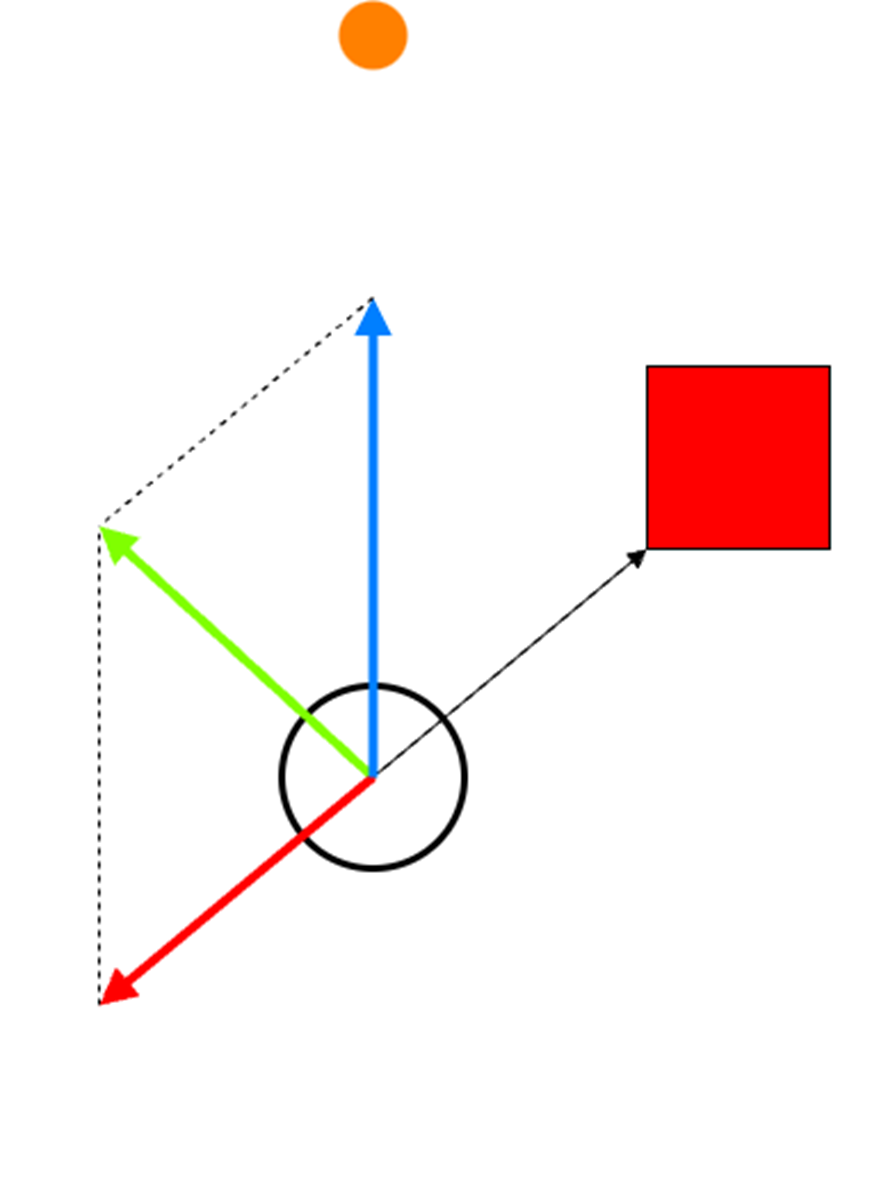
\includegraphics[width=0.95\linewidth,height=0.58\textheight,keepaspectratio]{images/tema_3/4_1_s05_ejercicio-practico_img01.png}
    \end{column}
  \end{columns}
\end{frame}

\section{Ejercicio práctico}

\section{Láser}

\begin{frame}{Mensajes de láser}
  \small
  \begin{columns}[T,onlytextwidth]
    \begin{column}{0.58\textwidth}
      \begin{itemize}
        \item Todos los láseres en ROS 2 publican el mismo tipo de mensajes
      \end{itemize}
    \end{column}
    \begin{column}{0.42\textwidth}
    \centering
    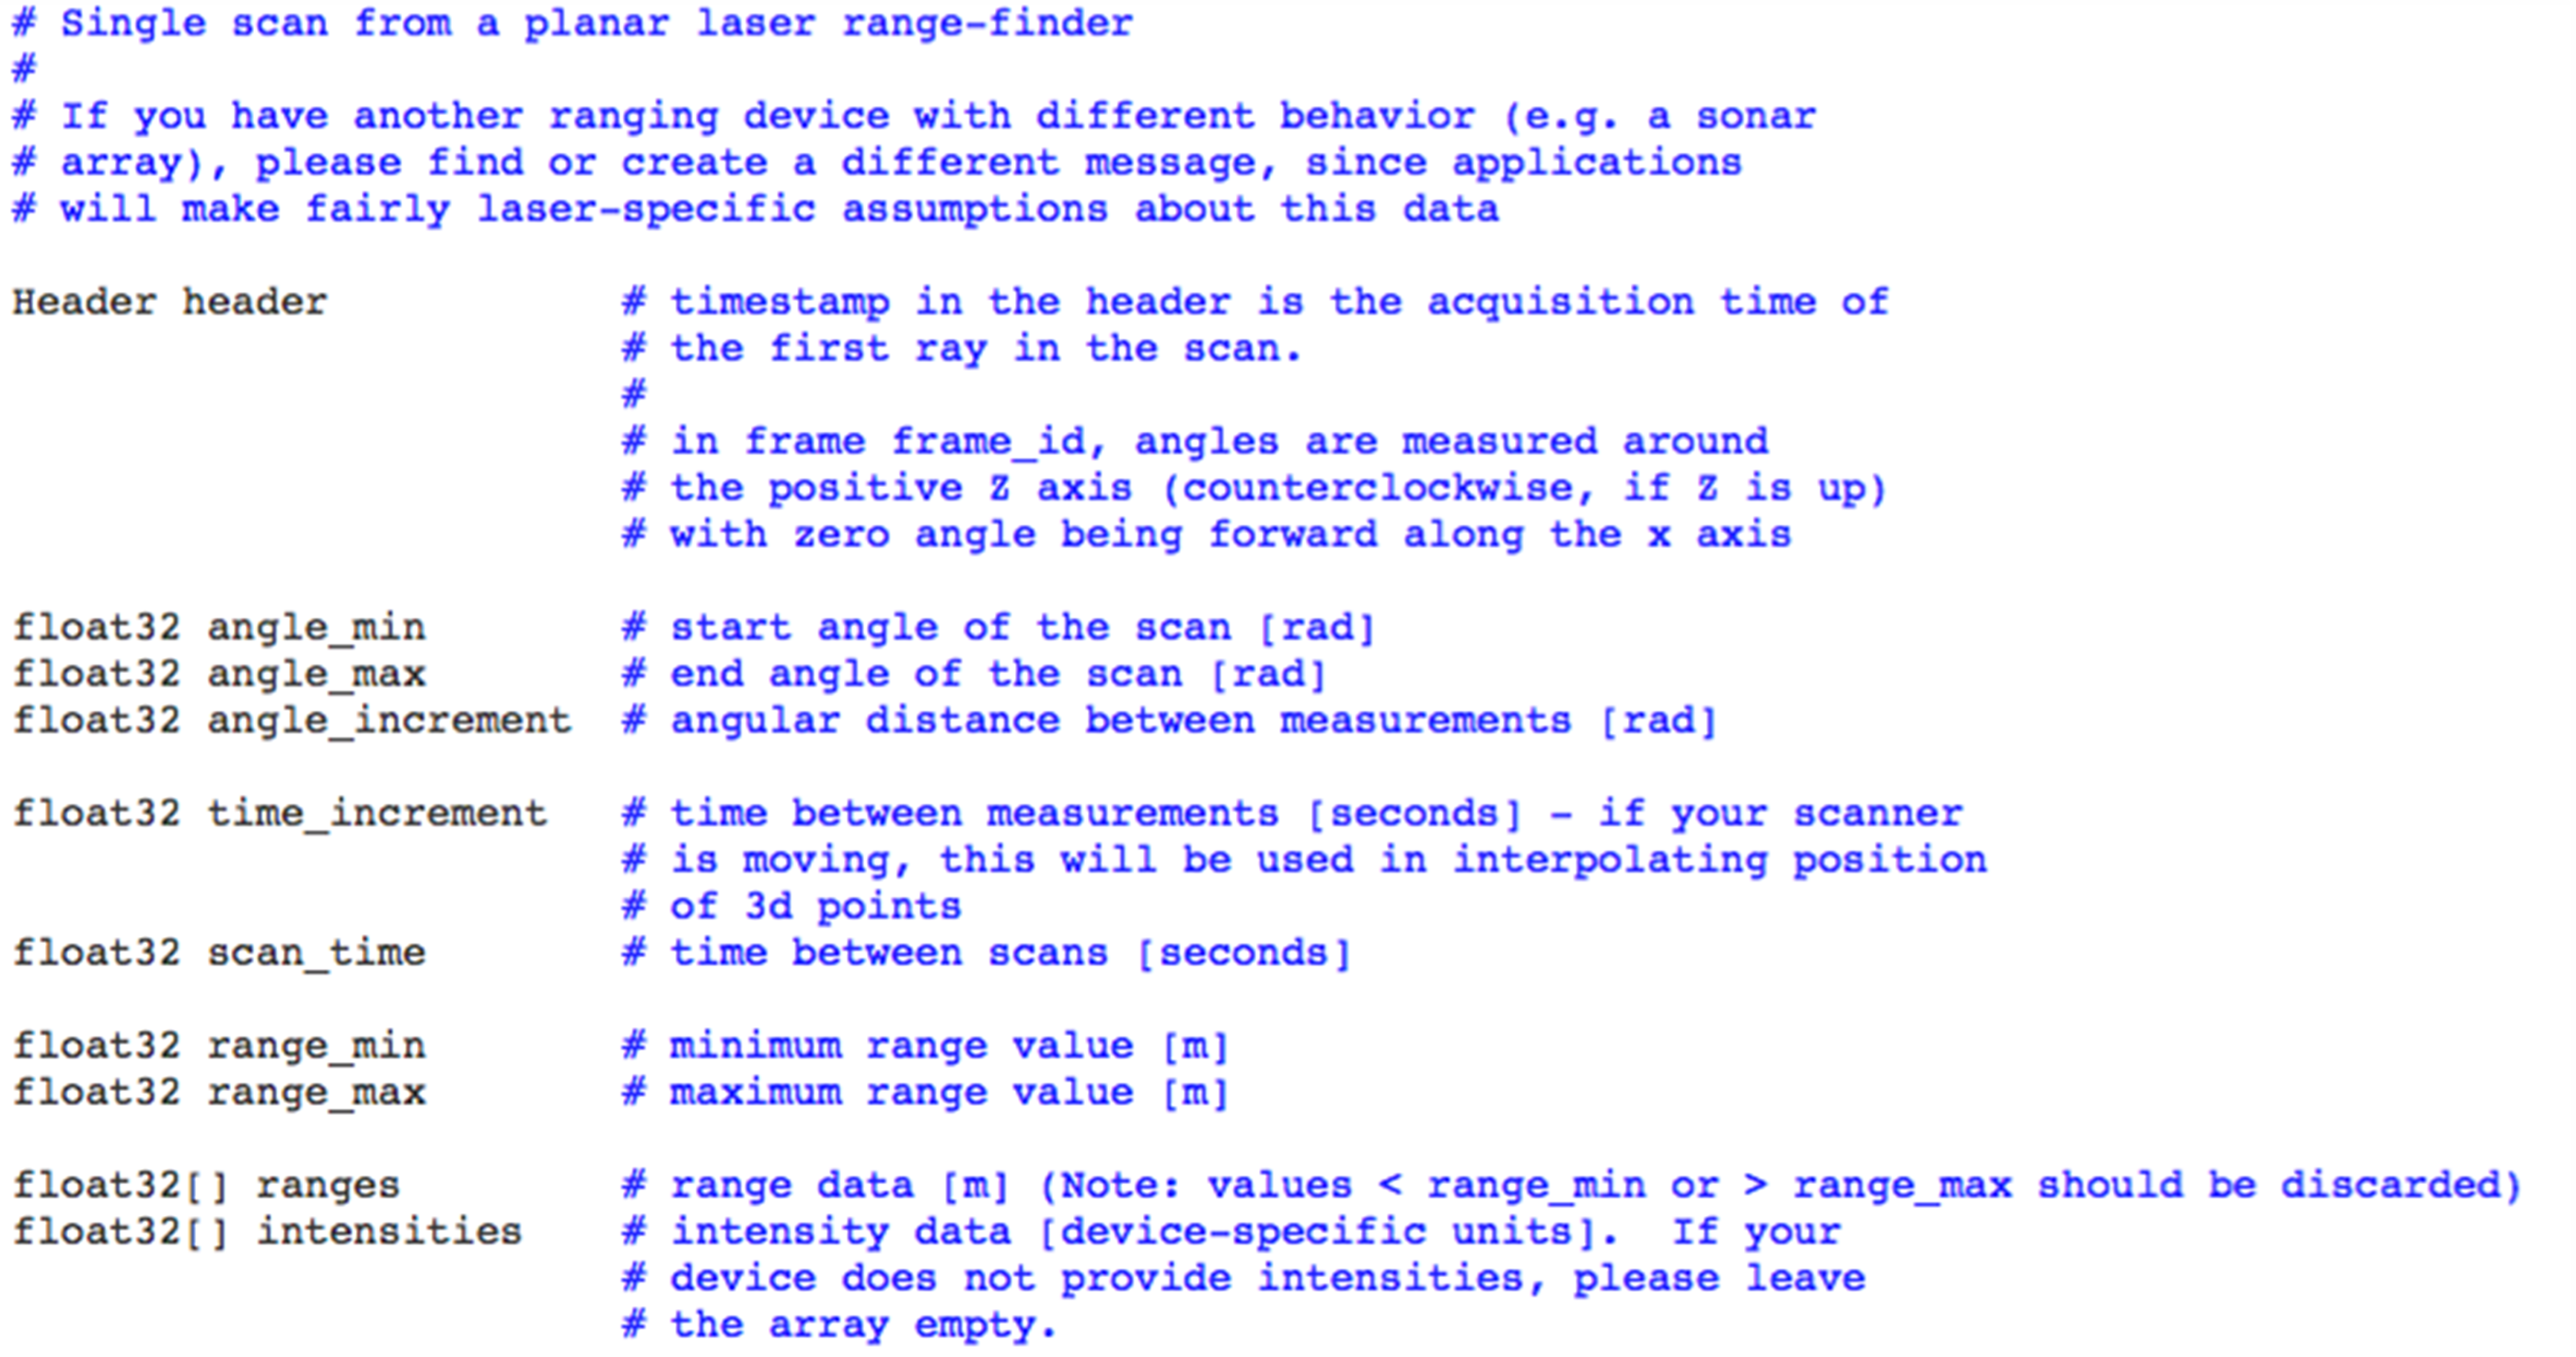
\includegraphics[width=0.95\linewidth,height=0.58\textheight,keepaspectratio]{images/tema_3/4_1_s08_mensajes-de-laser_img01.png}
    \end{column}
  \end{columns}
\end{frame}

\begin{frame}{Mensajes de láser en ROS 2}
  \small
  \begin{itemize}
    \item Tipo estándar: \textbf{sensor\_msgs/msg/LaserScan}.
    \item Ángulo del rayo $i$:
    \[
      \theta_i = \texttt{angle\_min} + i\cdot\texttt{angle\_increment}
    \]
    \item Conversión polar-cartesiana:
    \[
      x_i=r_i\cos(\theta_i),\quad y_i=r_i\sin(\theta_i)
    \]
    \item Cada rayo tiene instante propio:
    \[
      t_i=t_0+i\cdot\texttt{time\_increment}
    \]
    \item Si el robot se mueve durante el barrido, ignorar el tiempo de cada rayo distorsiona la geometría.
  \end{itemize}
\end{frame}

\begin{frame}{Mensajes de láser}
  \small
  \begin{columns}[T,onlytextwidth]
    \begin{column}{0.58\textwidth}
      \begin{itemize}
        \item Ejemplo:
        \item angle\_min=-Pi 360º
        \item angle\_max=Pi
        \item angle\_increment=2*Pi/100
        \item range\_min=0.05
        \item range\_max=20.0
      \end{itemize}
    \end{column}
    \begin{column}{0.42\textwidth}
    \centering
    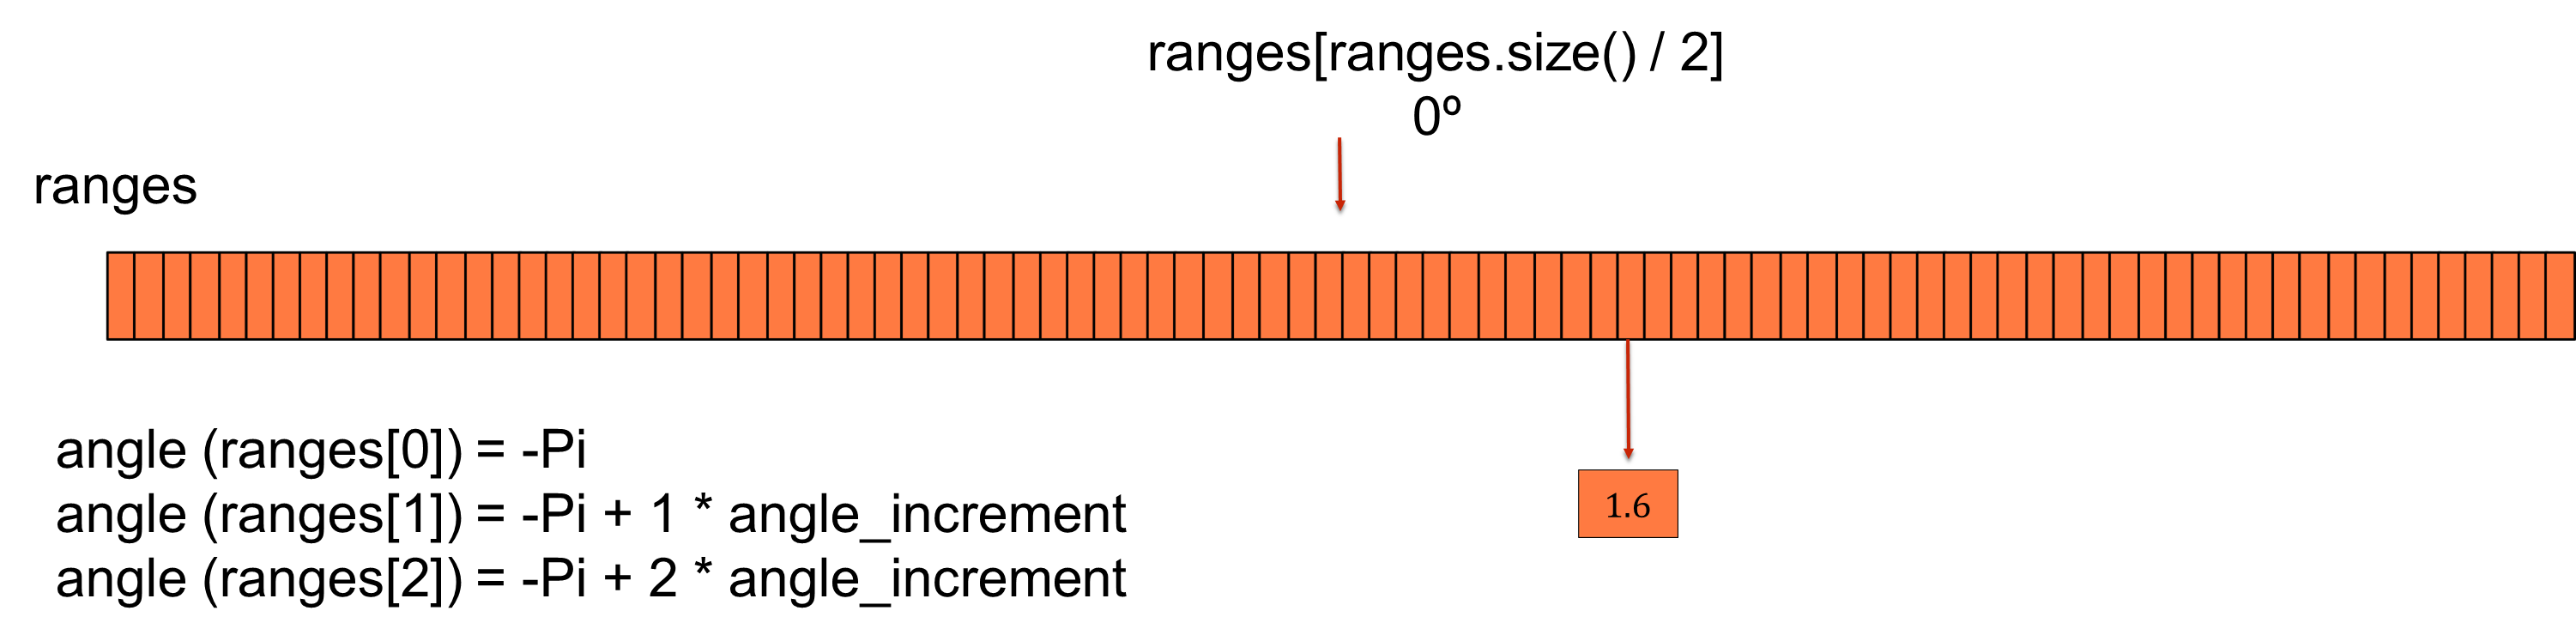
\includegraphics[width=0.95\linewidth,height=0.58\textheight,keepaspectratio]{images/tema_3/4_1_s09_mensajes-de-laser_img01.png}
    \end{column}
  \end{columns}
\end{frame}

\section{Ejemplo (sensors)}

\section{Ejercicio práctico}

\section{Cámaras}

\begin{frame}{Visión artificial}
  \small
  \begin{columns}[T,onlytextwidth]
    \begin{column}{0.58\textwidth}
      \begin{itemize}
        \item Las cámaras imitan los ojos
        \item Principio de funcionamiento: la luz reflejada en los objetos pasa a través de una lente (iris) en un plano de la imagen (retina) formando una imagen que puede ser procesada
      \end{itemize}
    \end{column}
    \begin{column}{0.42\textwidth}
    \centering
    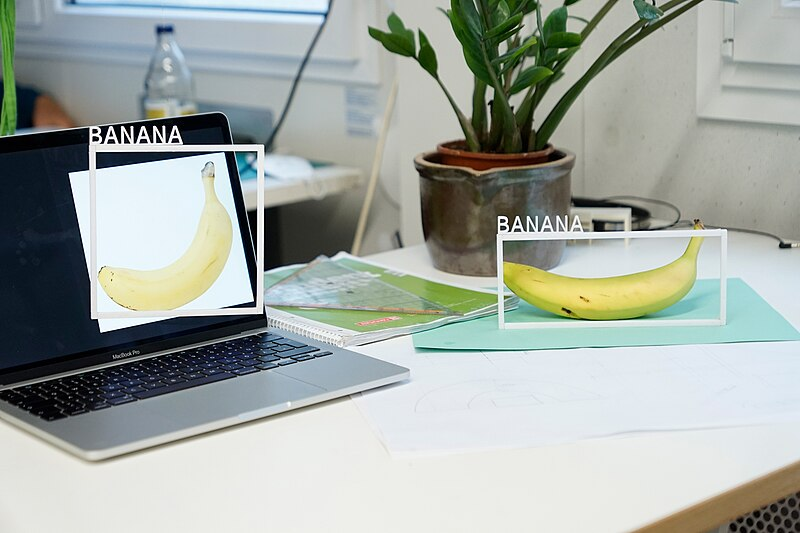
\includegraphics[width=0.95\linewidth,height=0.58\textheight,keepaspectratio]{images/tema_3/4_1_s13_vision-artificial_img01.jpeg}
    \end{column}
  \end{columns}
\end{frame}

\begin{frame}{Visión artificial}
  \small
  \begin{columns}[T,onlytextwidth]
    \begin{column}{0.58\textwidth}
      \begin{itemize}
        \item ¿Qué se puede hacer?
        \item Extracción de bordes
        \item Filtrado por color
        \item Segmentación de objetos
        \item Reconocimiento de formas, caras, etc.
        \item Reconstrucción 3D •…
        \item Aplicaciones generales:
        \item Medicina
        \item Biometría
        \item Ojo de halcón (tenis) •…
      \end{itemize}
    \end{column}
    \begin{column}{0.42\textwidth}
    \centering
    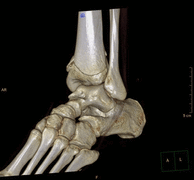
\includegraphics[width=0.95\linewidth,height=0.58\textheight,keepaspectratio]{images/tema_3/4_1_s14_vision-artificial_img01.png}
    \end{column}
  \end{columns}
\end{frame}

\begin{frame}{Tipos de cámaras}
  \small
  \begin{itemize}
    \item Cámaras estéreo (Bumblebee)
    \item Cámaras RGBD (Kinect, Xtion, Kinect2)
    \item Software de visión $\rightarrow$ OpenCV
  \end{itemize}
\end{frame}

\begin{frame}{Visión artificial en robótica}
  \small
  \begin{itemize}
    \item Es un sensor más que proporciona información del entorno
    \item Potencialmente muy rico
    \item Muy barato
    \item Muy utilizado
    \item Genera muchos datos $\rightarrow$ que hay que procesar
    \item Tiempo real
    \item Robustez
  \end{itemize}
\end{frame}

\begin{frame}{Visión artificial en robótica}
  \small
  \begin{columns}[T,onlytextwidth]
    \begin{column}{0.58\textwidth}
      \begin{itemize}
        \item Aplicaciones:
        \item Navegación (!)
        \item Control visual
        \item Mapeado
        \item Auto-localización
        \item Identificación de objetos para realizar diferentes operaciones
        \item Conducción autónoma (reconocimiento de señales, semáforos, líneas, etc.) •…
      \end{itemize}
    \end{column}
    \begin{column}{0.42\textwidth}
    \centering
    
\includegraphics[width=0.95\linewidth,height=0.58\textheight,keepaspectratio]{images/tema_3/4_1_s17_tipos-de-camaras_img01.png}
    \end{column}
  \end{columns}
\end{frame}

\begin{frame}{Imagen digital}
  \small
  \begin{columns}[T,onlytextwidth]
    \begin{column}{0.58\textwidth}
      \begin{itemize}
        \item El plano se divide en partes iguales (píxeles), normalmente rectangulares
        \item Resolución:
        \item Cámaras $\rightarrow$ 640x480 (por ejemplo)
        \item Ojo humano $\rightarrow$ 120x106x6x106 terminaciones nerviosas
        \item El valor de cada píxel el proporcional a la cantidad de luz reflejada por la parte de la superficie del objeto que se proyecta en ese píxel:
        \item Material del objeto
        \item Iluminación de la escena
        \item Reflejo de otros objetos
      \end{itemize}
    \end{column}
    \begin{column}{0.42\textwidth}
    \centering
    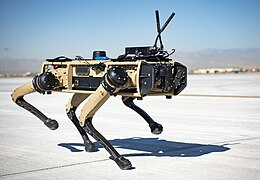
\includegraphics[width=0.95\linewidth,height=0.58\textheight,keepaspectratio]{images/tema_3/4_1_s18_vision-artificial-en-robotica_img01.jpeg}
    \end{column}
  \end{columns}
\end{frame}

\begin{frame}{Procesamiento básico}
  \small
  \begin{columns}[T,onlytextwidth]
    \begin{column}{0.58\textwidth}
      \begin{itemize}
        \item Conversión a escala de grises • Segmentación
        \item Filtros de color • Regiones de interés
        \item Filtros de bordes •…
        \item Filtros de esquinas
        \item Convoluciones
        \item Flujo óptico
        \item Erosión
        \item Dilatación
        \item Extracción de líneas
      \end{itemize}
    \end{column}
    \begin{column}{0.42\textwidth}
    \centering
    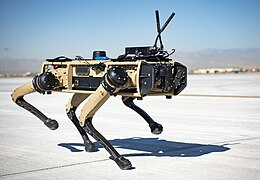
\includegraphics[width=0.95\linewidth,height=0.58\textheight,keepaspectratio]{images/tema_3/4_1_s19_vision-artificial-en-robotica_img01.jpeg}
    \end{column}
  \end{columns}
\end{frame}

\begin{frame}{Formatos}
  \small
  \begin{columns}[T,onlytextwidth]
    \begin{column}{0.58\textwidth}
      \begin{itemize}
        \item Niveles de gris
        \item Color sin compresión:
        \item RGB $\rightarrow$ mezcla cromaticidad con iluminación
        \item HSV $\rightarrow$ tono + saturación + intensidad
        \item Color con compresión:
        \item JPEG
        \item PNG •…
      \end{itemize}
    \end{column}
    \begin{column}{0.42\textwidth}
    \centering
    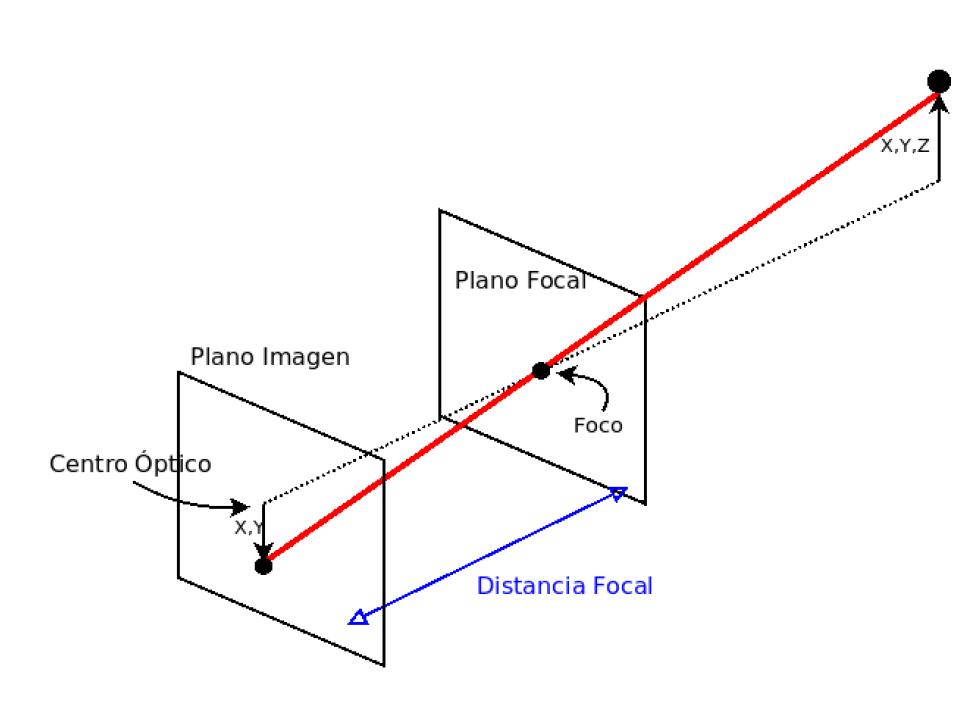
\includegraphics[width=0.97\linewidth,height=0.26\textheight,keepaspectratio]{images/tema_3/4_1_s20_formacion-de-la-imagen_img01.png}
    \par\vspace{0.02\textheight}
    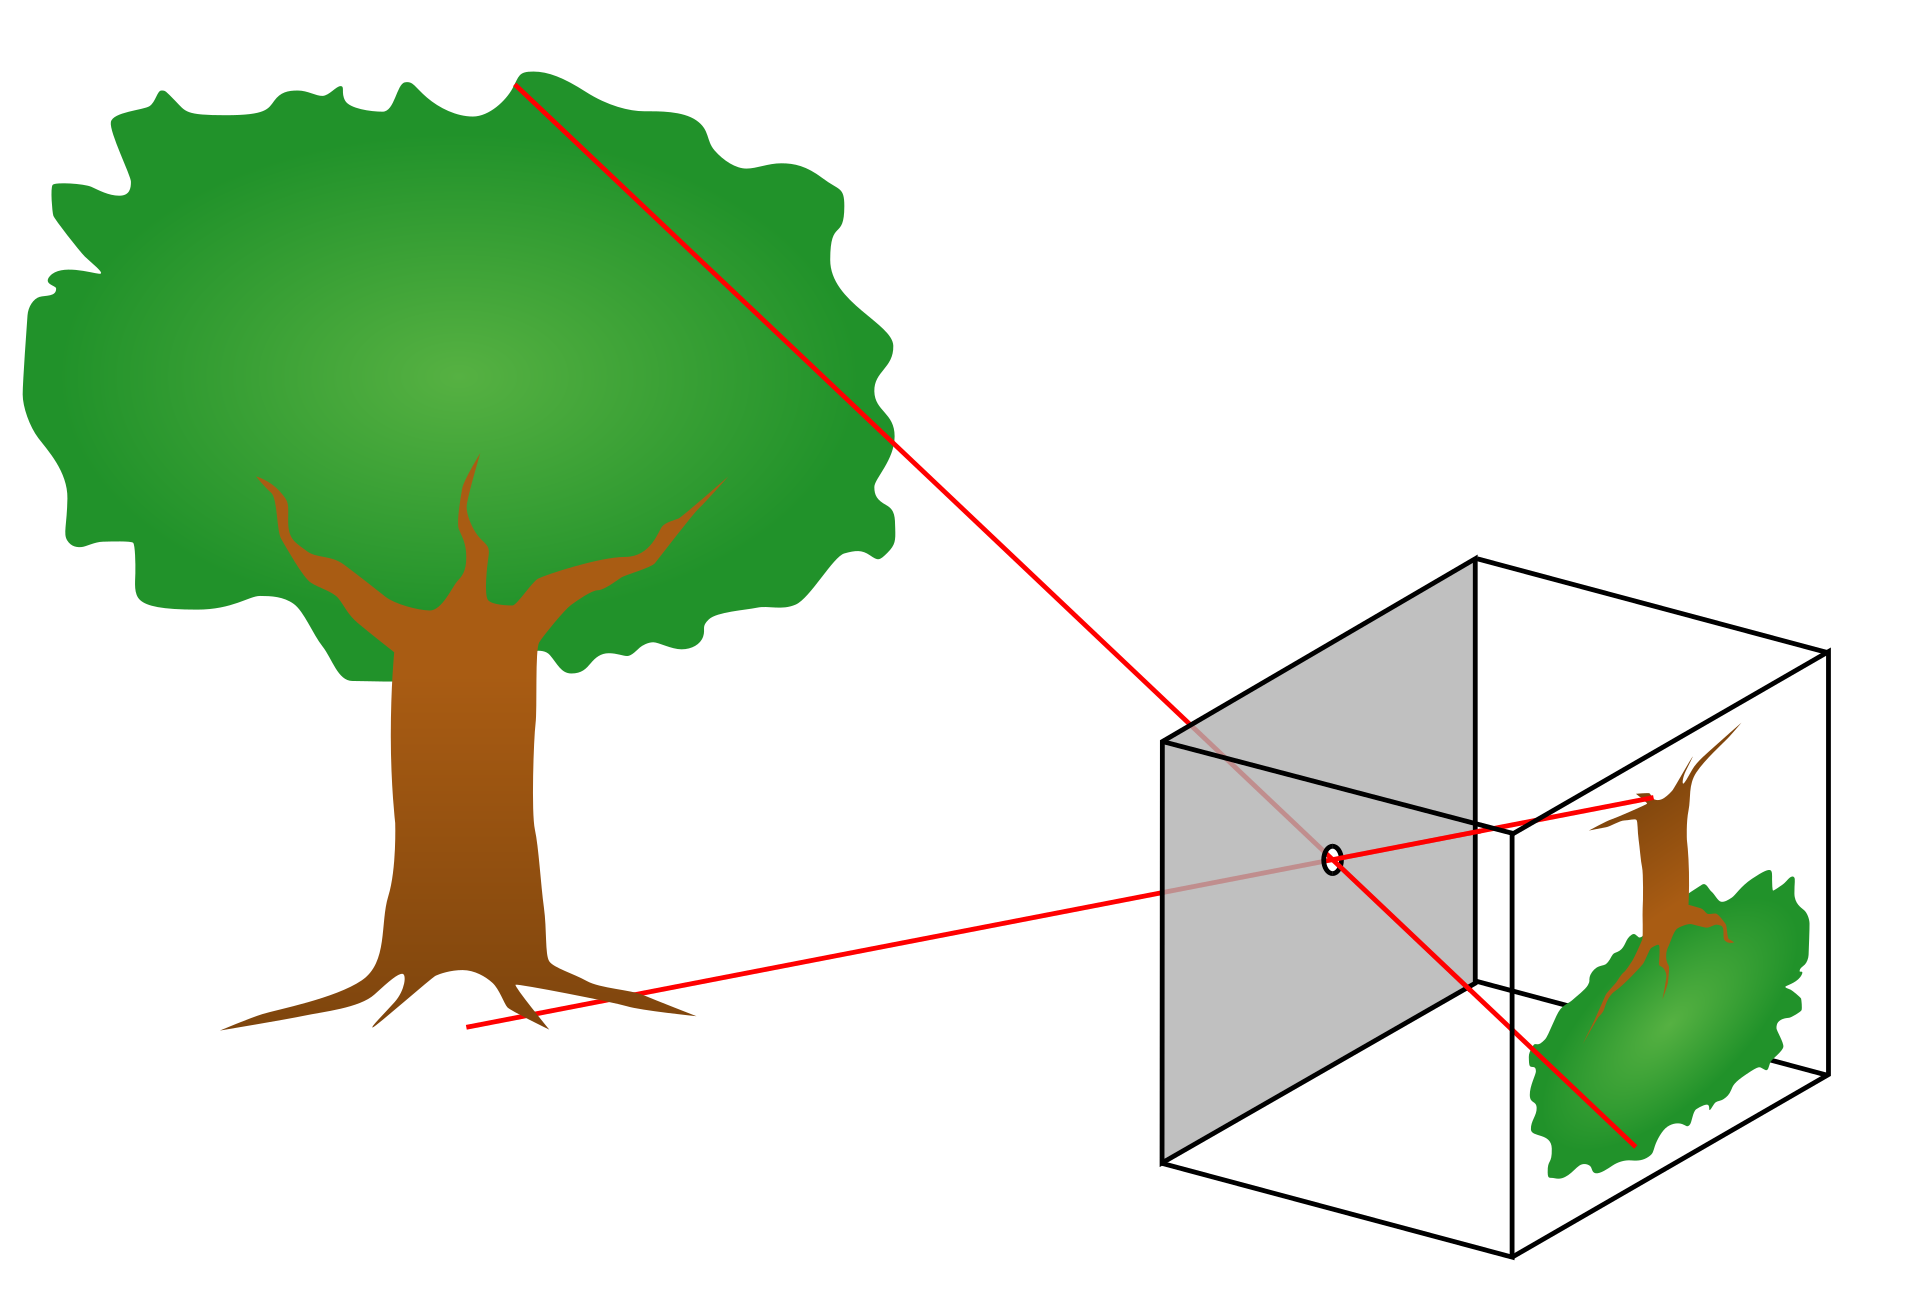
\includegraphics[width=0.97\linewidth,height=0.26\textheight,keepaspectratio]{images/tema_3/4_1_s20_formacion-de-la-imagen_img02.png}
    \end{column}
  \end{columns}
\end{frame}

\begin{frame}{Ejemplo de control visual: seguimiento de}
  \small
  \begin{columns}[T,onlytextwidth]
    \begin{column}{0.58\textwidth}
      \begin{itemize}
        \item objetos
      \end{itemize}
      \begin{itemize}
        \item Percepción $\rightarrow$ identificar el objeto
        \item Actuación $\rightarrow$ corregir la orientación y la velocidad de avance
      \end{itemize}
    \end{column}
    \begin{column}{0.42\textwidth}
    \centering
    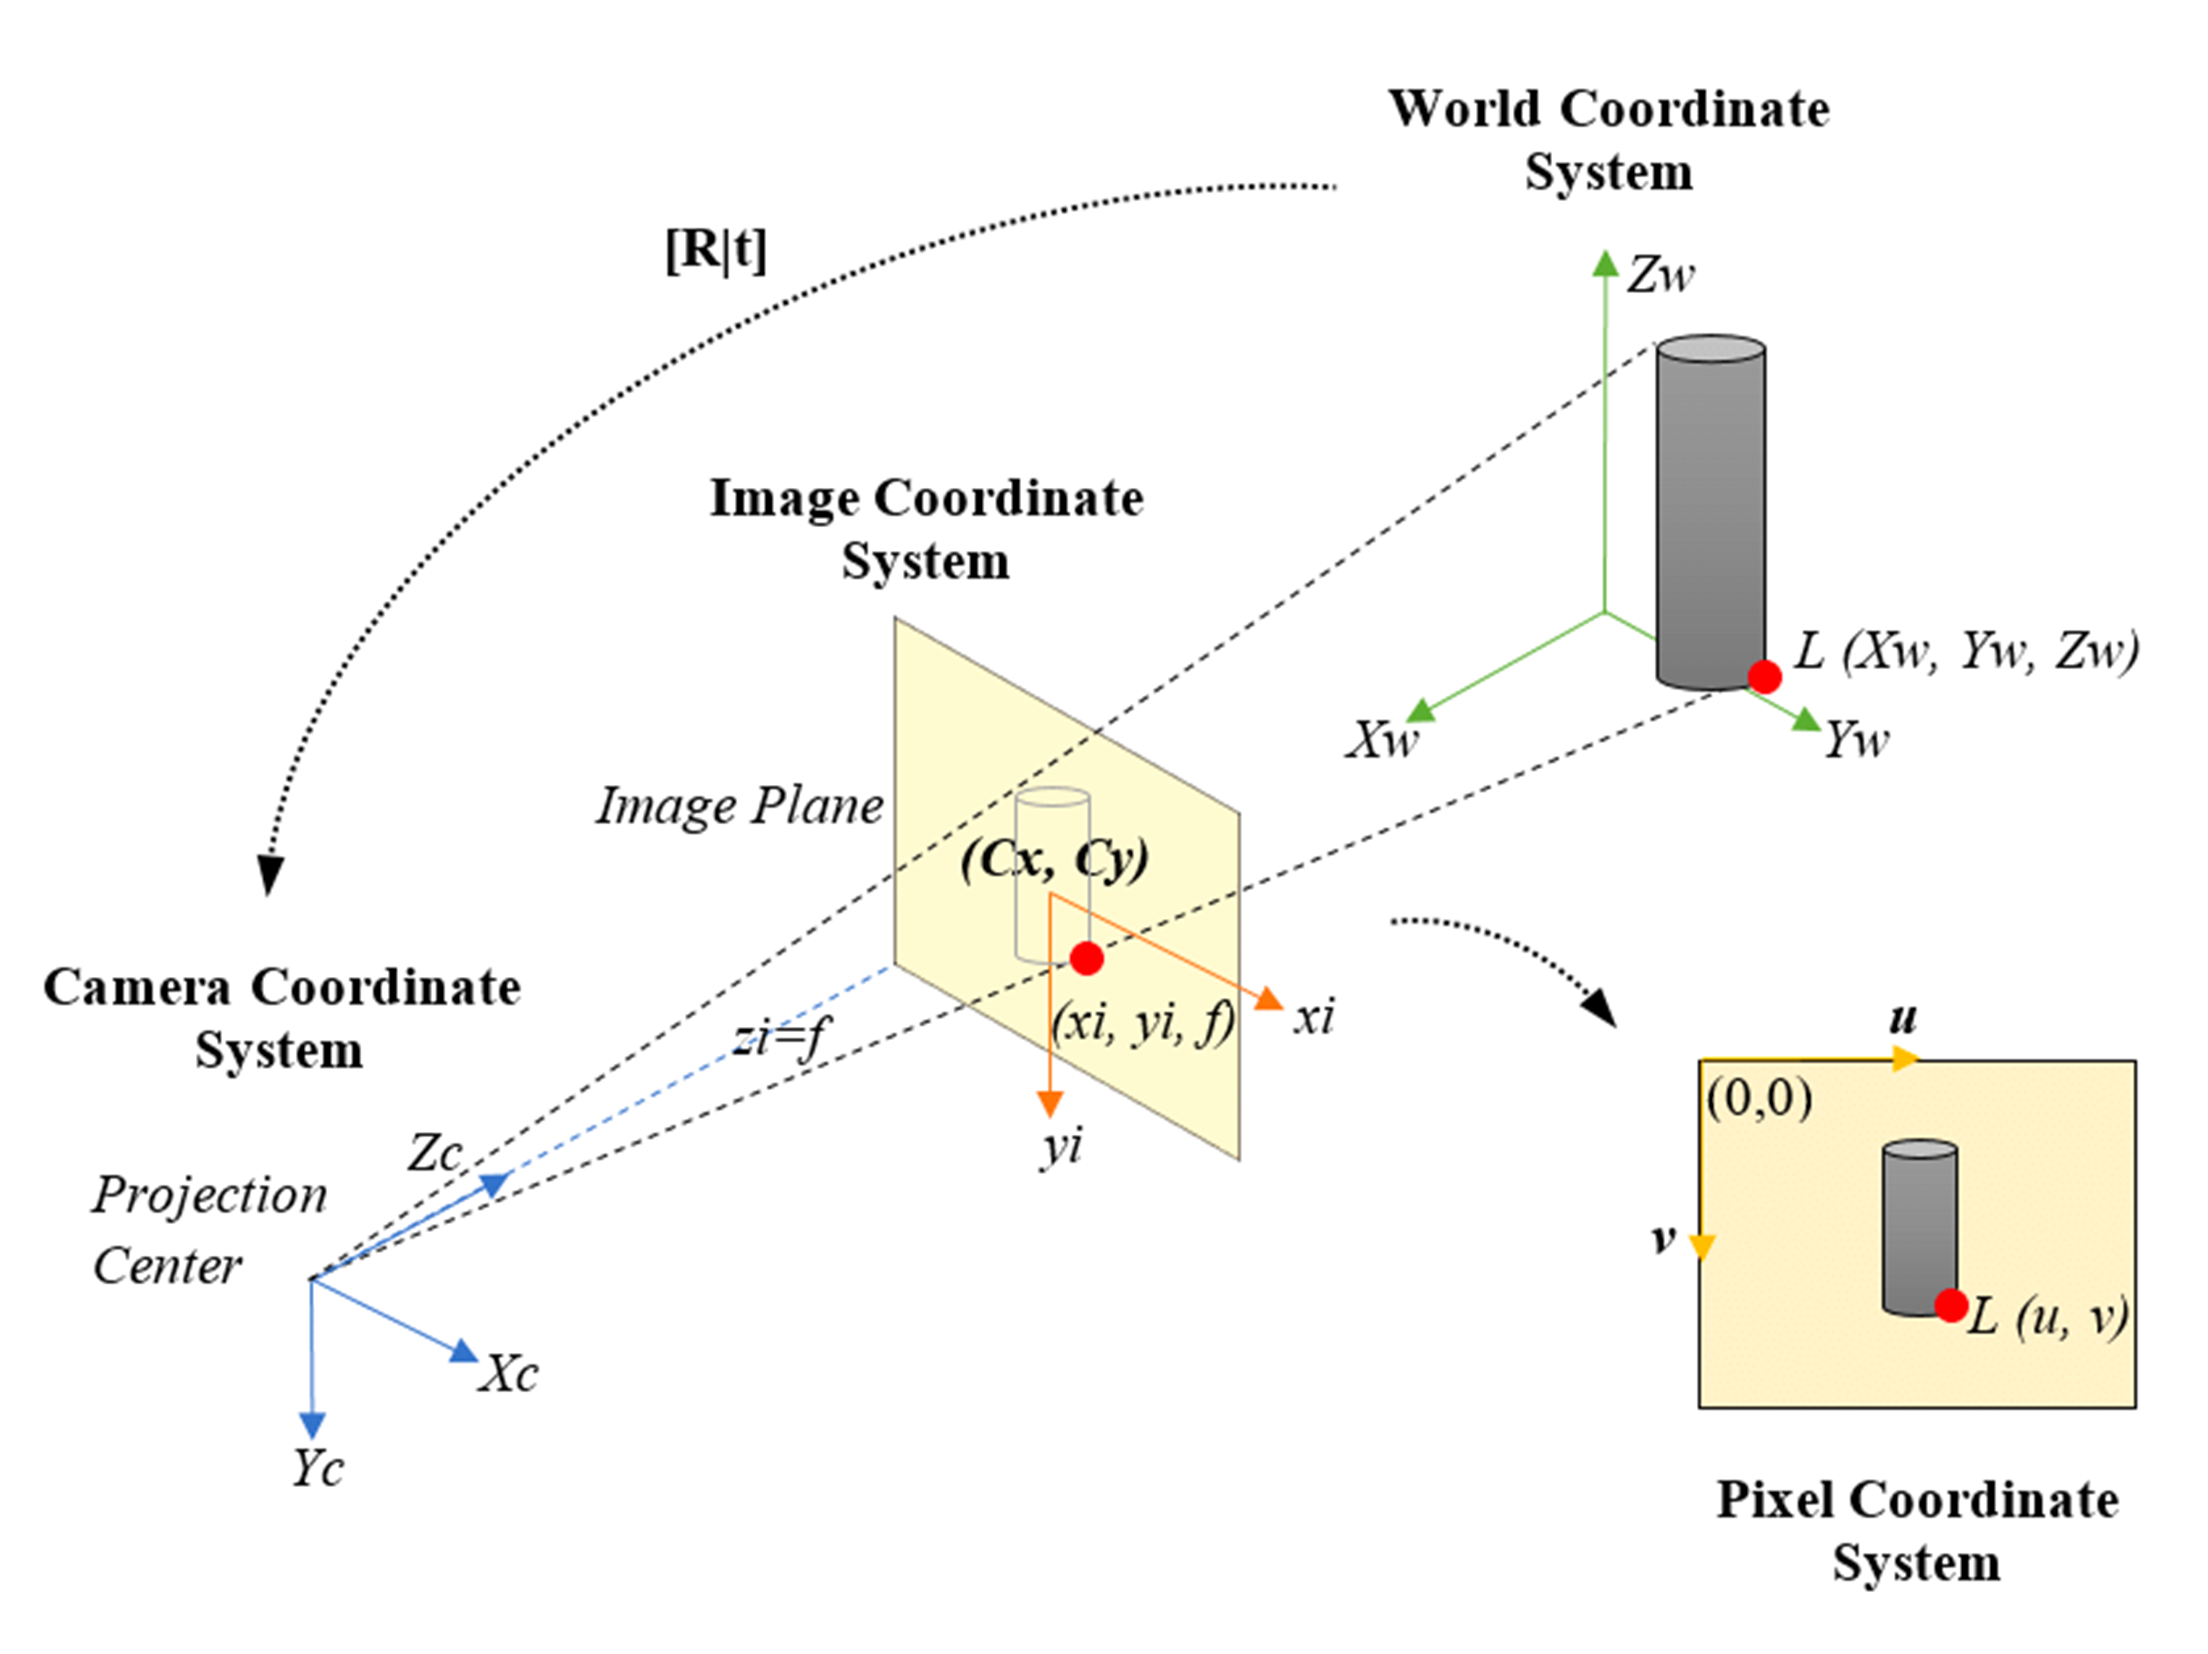
\includegraphics[width=0.95\linewidth,height=0.58\textheight,keepaspectratio]{images/tema_3/4_1_s21_formacion-de-la-imagen_img01.png}
    \end{column}
  \end{columns}
\end{frame}

\section{Imagen}

\section{Ejemplo}

\begin{frame}{Mensajes de imagen}
  \small
  \begin{columns}[T,onlytextwidth]
    \begin{column}{0.58\textwidth}
      \begin{itemize}
        \item Todas las cámaras en ROS 2 publican el mismo tipo de mensajes
      \end{itemize}
    \end{column}
    \begin{column}{0.42\textwidth}
    \centering
    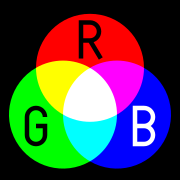
\includegraphics[width=0.97\linewidth,height=0.26\textheight,keepaspectratio]{images/tema_3/4_1_s24_formatos_img01.png}
    \par\vspace{0.02\textheight}
    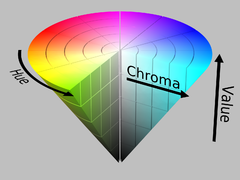
\includegraphics[width=0.97\linewidth,height=0.26\textheight,keepaspectratio]{images/tema_3/4_1_s24_formatos_img02.png}
    \end{column}
  \end{columns}
\end{frame}

\begin{frame}{Trabajar con imágenes}
  \small
  \begin{columns}[T,onlytextwidth]
    \begin{column}{0.58\textwidth}
      \begin{itemize}
        \item Las imágenes las procesamos utilizando OpenCV (estándar)
        \item Tipo principal $\rightarrow$ cv::Mat
        \item cv::Mat transforma sensor\_msgs::msgs::Image a cv::Mat
      \end{itemize}
    \end{column}
    \begin{column}{0.42\textwidth}
    \centering
    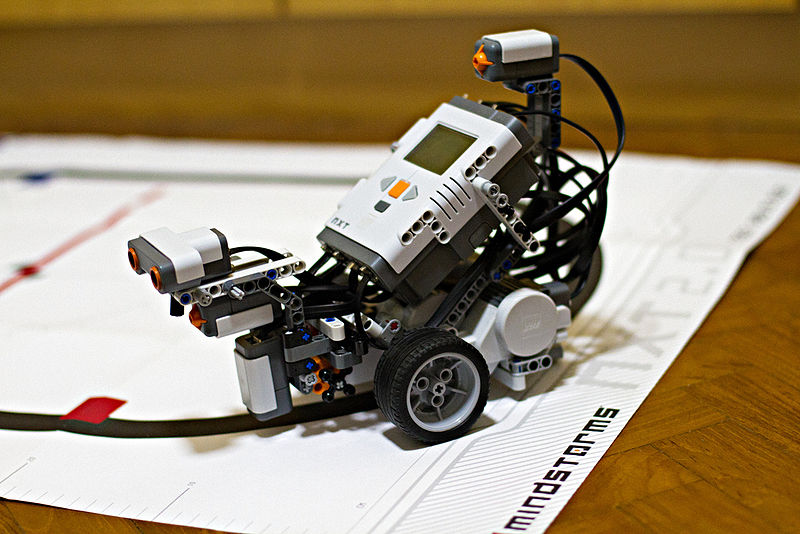
\includegraphics[width=0.95\linewidth,height=0.58\textheight,keepaspectratio]{images/tema_3/4_1_s25_ejemplo-de-control-visual-seguimiento-de-objetos_img01.jpeg}
    \end{column}
  \end{columns}
\end{frame}

\begin{frame}{Trabajar con imágenes}
  \small
  \begin{itemize}
    \item Las imágenes las procesamos utilizando OpenCV (estándar)
    \item Tipo principal $\rightarrow$ cv::Mat
    \item cv::Mat transforma sensor\_msgs::msgs::Image a cv::Mat
  \end{itemize}
\end{frame}

\begin{frame}{Modelo pin hole}
  \small
  \begin{columns}[T,onlytextwidth]
    \begin{column}{0.58\textwidth}
      \begin{itemize}
        \item Parámetros intrínsecos y extrínsecos de la cámara
        \item Valores por defecto vs. Calibración
        \item sensor:msgs::msg::CameraInfo
      \end{itemize}
    \end{column}
    \begin{column}{0.42\textwidth}
    \centering
    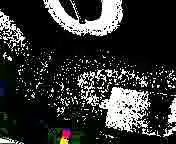
\includegraphics[width=0.95\linewidth,height=0.58\textheight,keepaspectratio]{images/tema_3/4_1_s27_ejemplo_img01.png}
    \end{column}
  \end{columns}
\end{frame}

\begin{frame}{Mensajes de imagen y calibración}
  \small
  \begin{itemize}
    \item Tipo estándar de imagen: \textbf{sensor\_msgs/msg/Image}.
    \item Campos clave: \texttt{height}, \texttt{width}, \texttt{encoding}, \texttt{step}, \texttt{data}.
    \item La calibración de cámara se publica en \textbf{sensor\_msgs/msg/CameraInfo}.
    \item La sincronización entre \texttt{Image}, \texttt{CameraInfo} y TF es crítica para percepción 3D y control visual.
    \item Para despliegues reales se suele usar compresión de transporte para reducir ancho de banda.
  \end{itemize}
\end{frame}

\section{Ejemplo (sensors)}

\begin{frame}{Percepción}
  \small
  \begin{columns}[T,onlytextwidth]
    \begin{column}{0.58\textwidth}
      \begin{itemize}
        \item VFF, láser e imagen
      \end{itemize}
    \end{column}
    \begin{column}{0.42\textwidth}
    \centering
    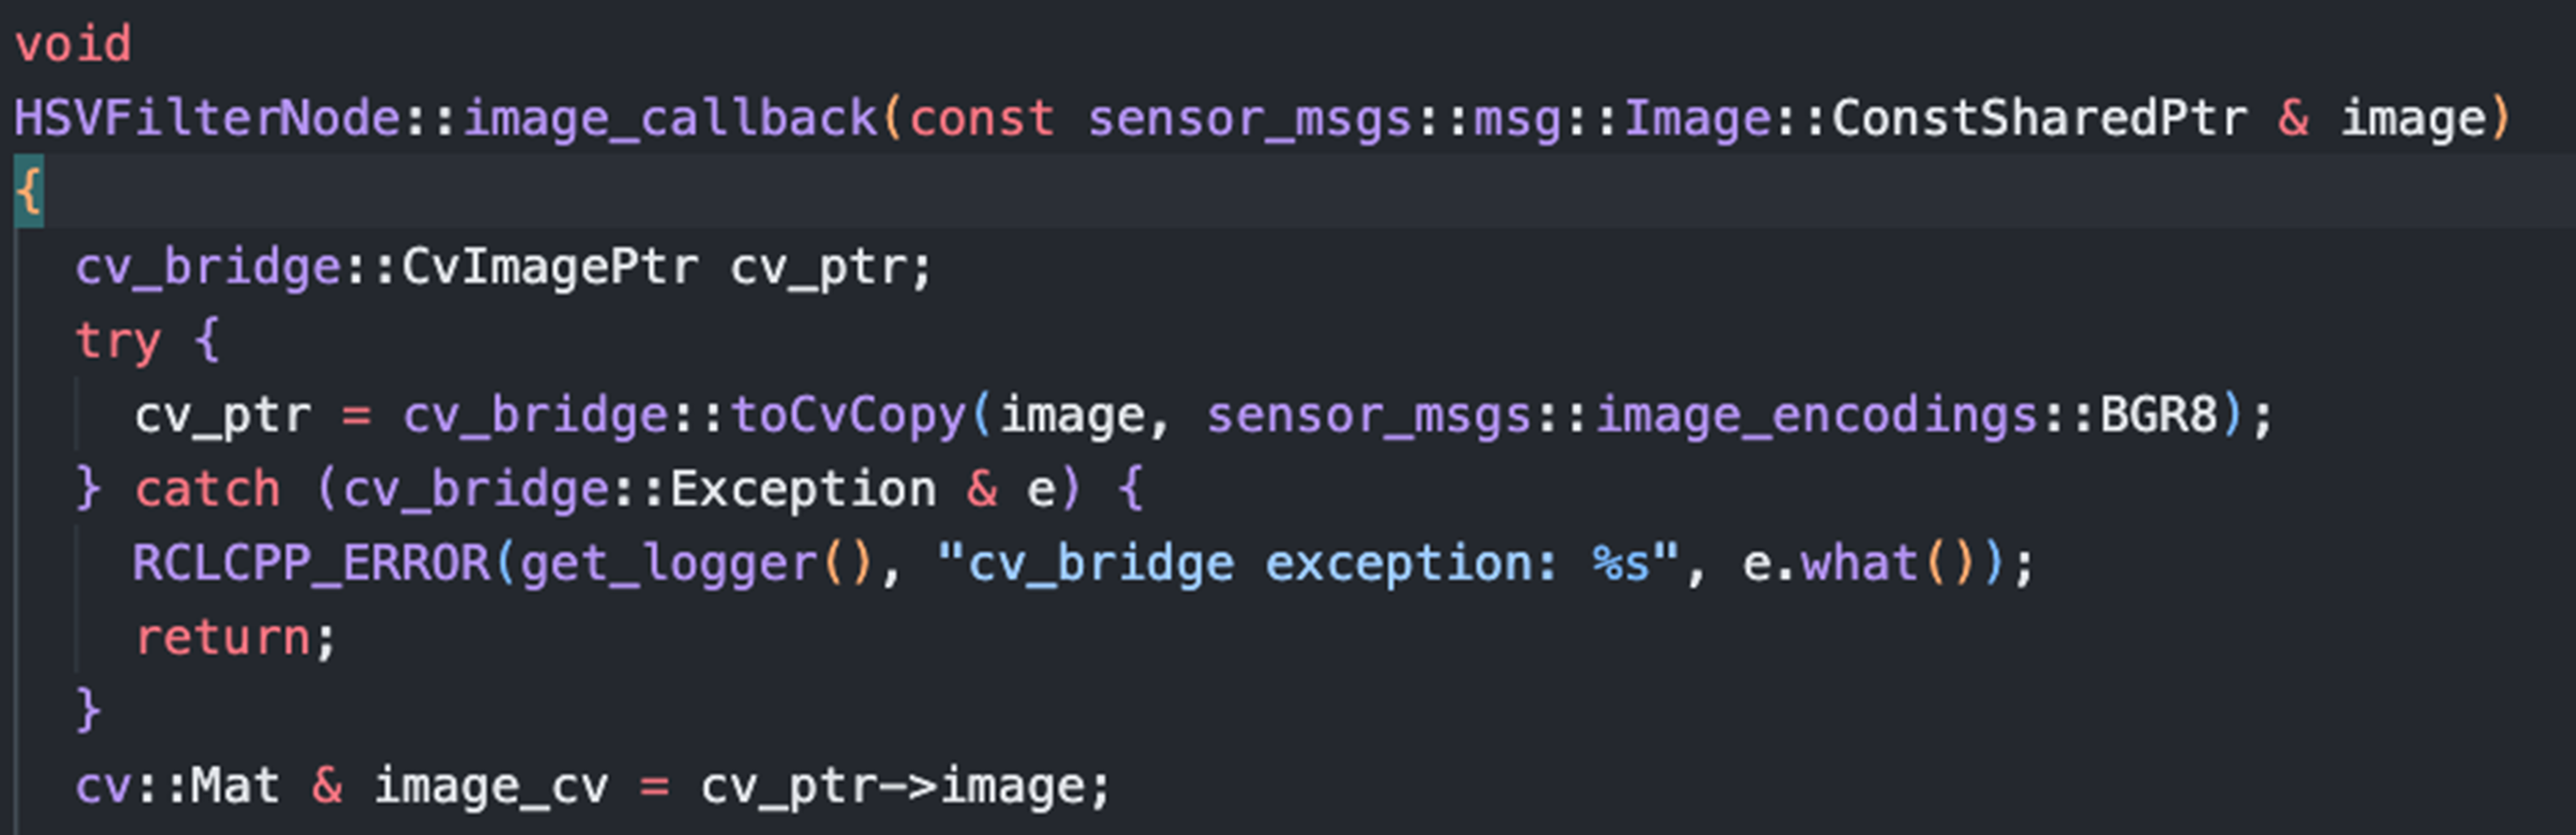
\includegraphics[width=0.95\linewidth,height=0.58\textheight,keepaspectratio]{images/tema_3/4_1_s29_trabajar-con-imagenes_img01.png}
    \end{column}
  \end{columns}
\end{frame}

\section{Percepción: deep learning y razonamiento espacial}

\section{Deep learning}

\begin{frame}{YOLOv8}
  \small
  \begin{columns}[T,onlytextwidth]
    \begin{column}{0.58\textwidth}
      \begin{itemize}
        \item Algoritmo de detección de objetos en imágenes y video
        \item Utiliza una red neuronal convolucional para predecir múltiples cajas delimitadoras y las probabilidades de clasificación correspondientes
        \item Aplicaciones:
        \item Robótica social
        \item Videovigilancia
        \item Conducción autónoma
        \item Drones •…
        \item Nvidia GPU + librerías CUDA
        \item Repo
      \end{itemize}
    \end{column}
    \begin{column}{0.42\textwidth}
    \centering
    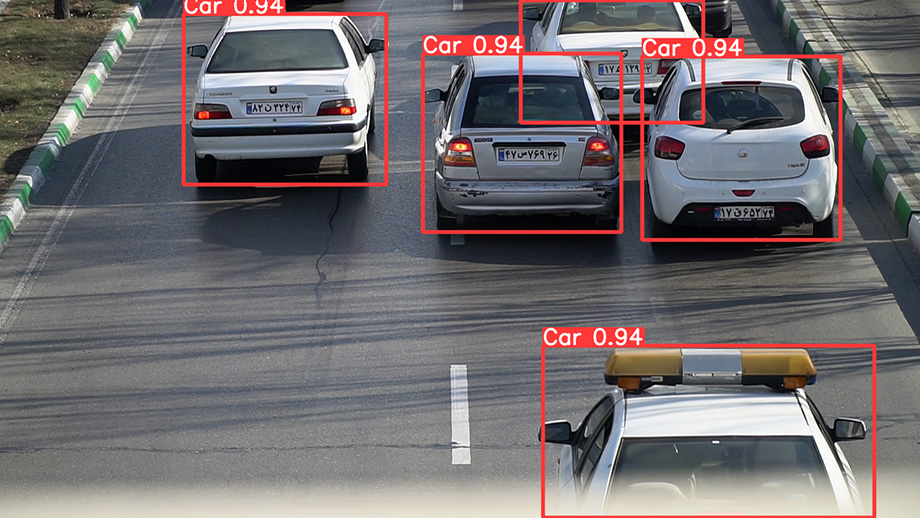
\includegraphics[width=0.95\linewidth,height=0.58\textheight,keepaspectratio]{images/tema_3/4_2_s03_yolov8_img01.png}
    \end{column}
  \end{columns}
\end{frame}

\begin{frame}{Detección de objetos}
  \small
  \begin{columns}[T,onlytextwidth]
    \begin{column}{0.58\textwidth}
      \begin{itemize}
        \item \$ ros2 launch yolov8\_bringup yolov8.launch.py
      \end{itemize}
      \begin{itemize}
        \item Se parte de un conjunto de datos (dataset):
        \item Conjunto de entrenamiento
        \item Conjunto de validación
      \end{itemize}
    \end{column}
    \begin{column}{0.42\textwidth}
    \centering
    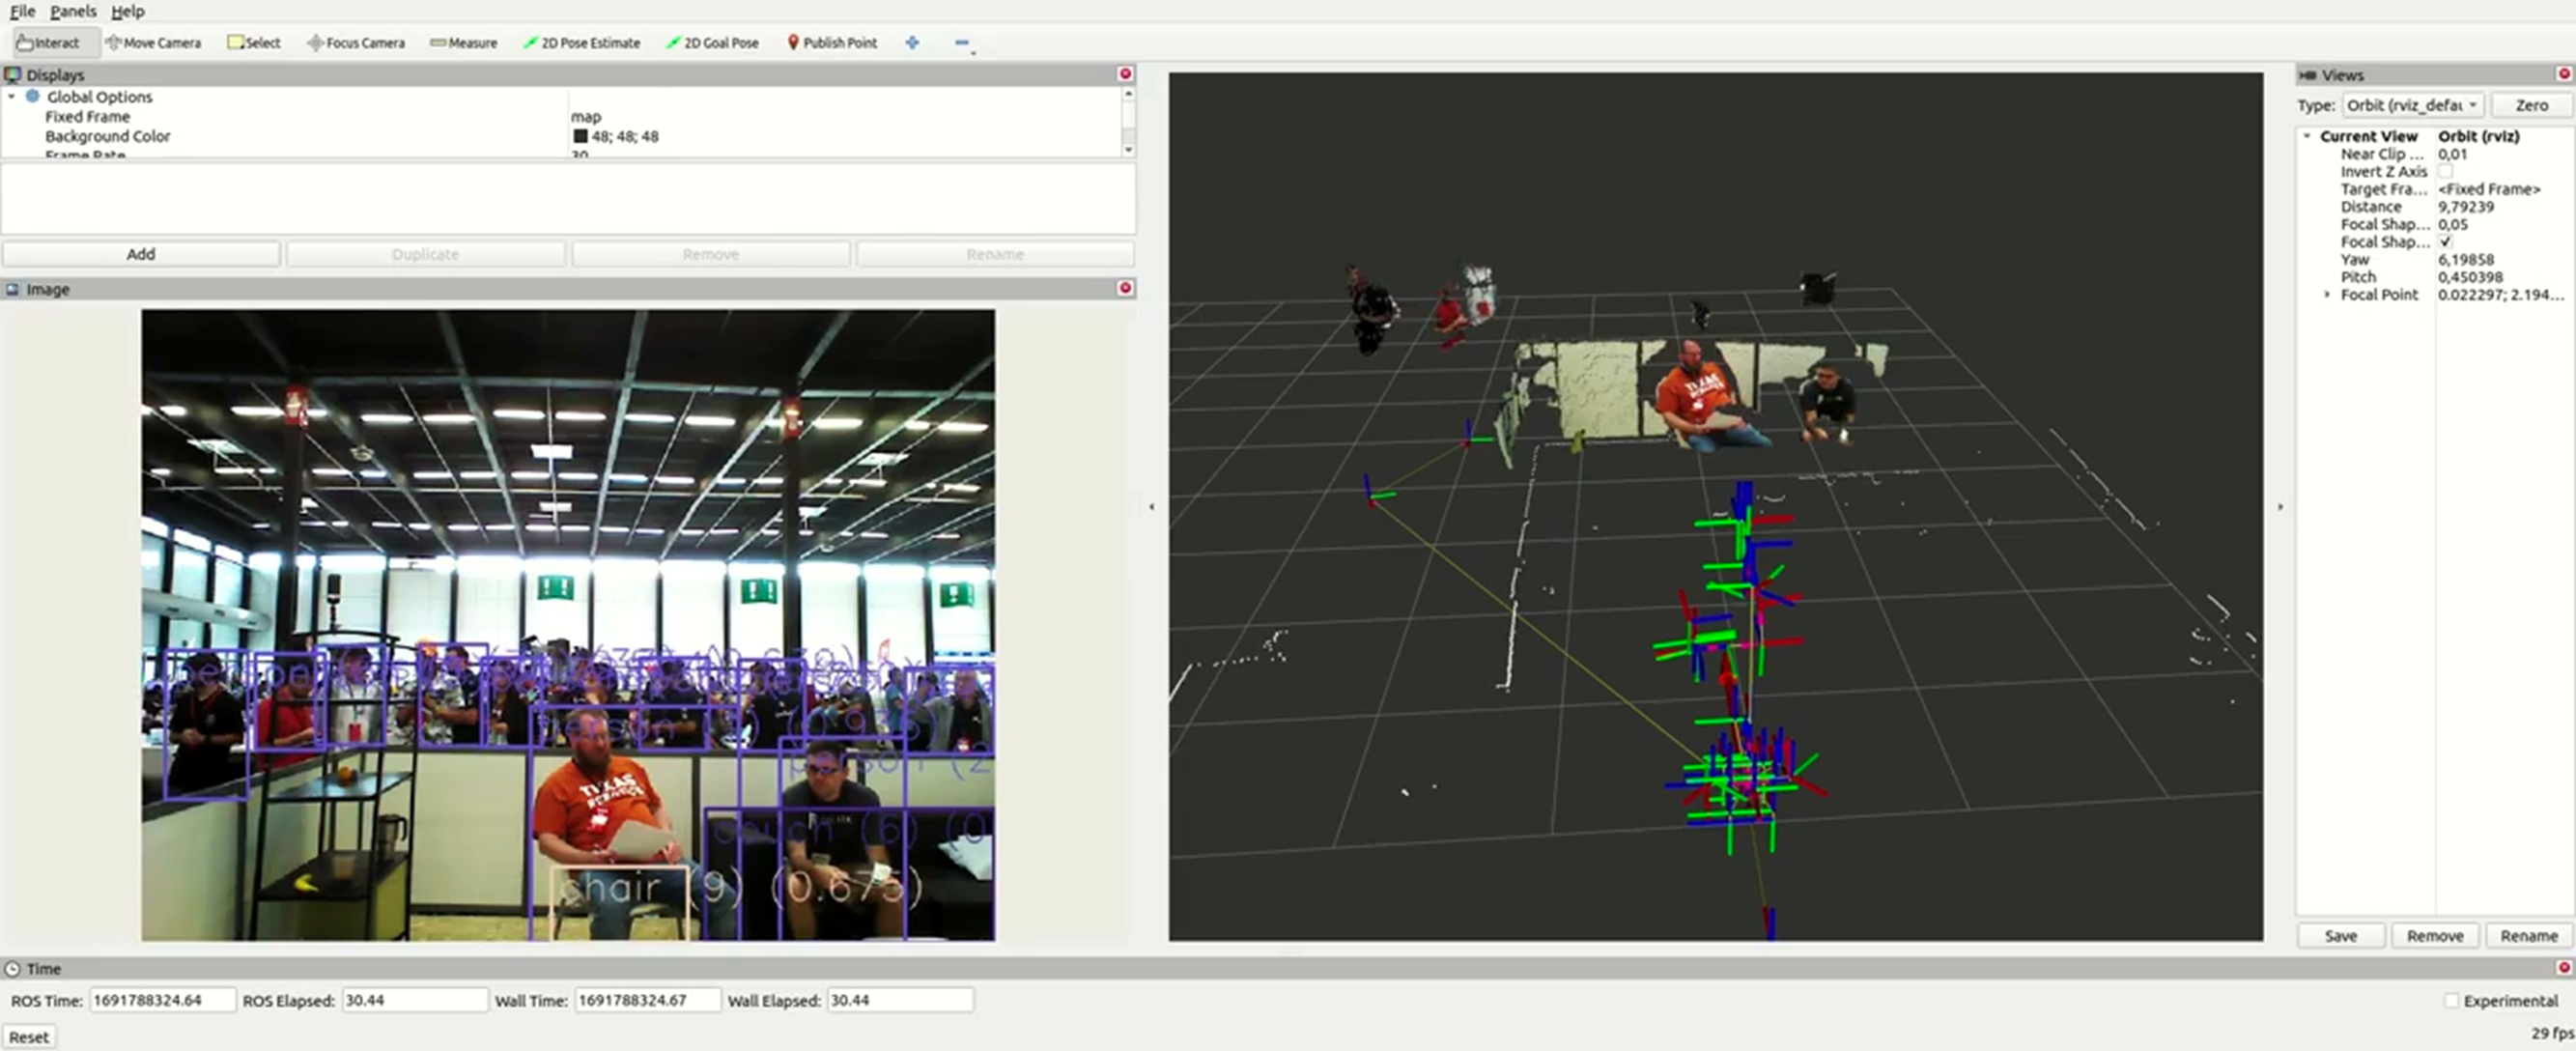
\includegraphics[width=0.95\linewidth,height=0.58\textheight,keepaspectratio]{images/tema_3/4_2_s04_deteccion-de-objetos_img01.png}
    \end{column}
  \end{columns}
\end{frame}

\begin{frame}{Detección de objetos: segmentación de}
  \small
  \begin{columns}[T,onlytextwidth]
    \begin{column}{0.58\textwidth}
      \begin{itemize}
        \item instancias
        \item \$ ros2 launch yolov8\_bringup yolov8.launch.py model:=src/sensors/models/yolov8m.pt image\_reliability:=1 input\_image\_topic:=/camera/color/image\_raw
      \end{itemize}
      \begin{itemize}
        \item Se parte de un conjunto de datos (dataset):
        \item Conjunto de entrenamiento
        \item Conjunto de validación
      \end{itemize}
    \end{column}
    \begin{column}{0.42\textwidth}
    \centering
    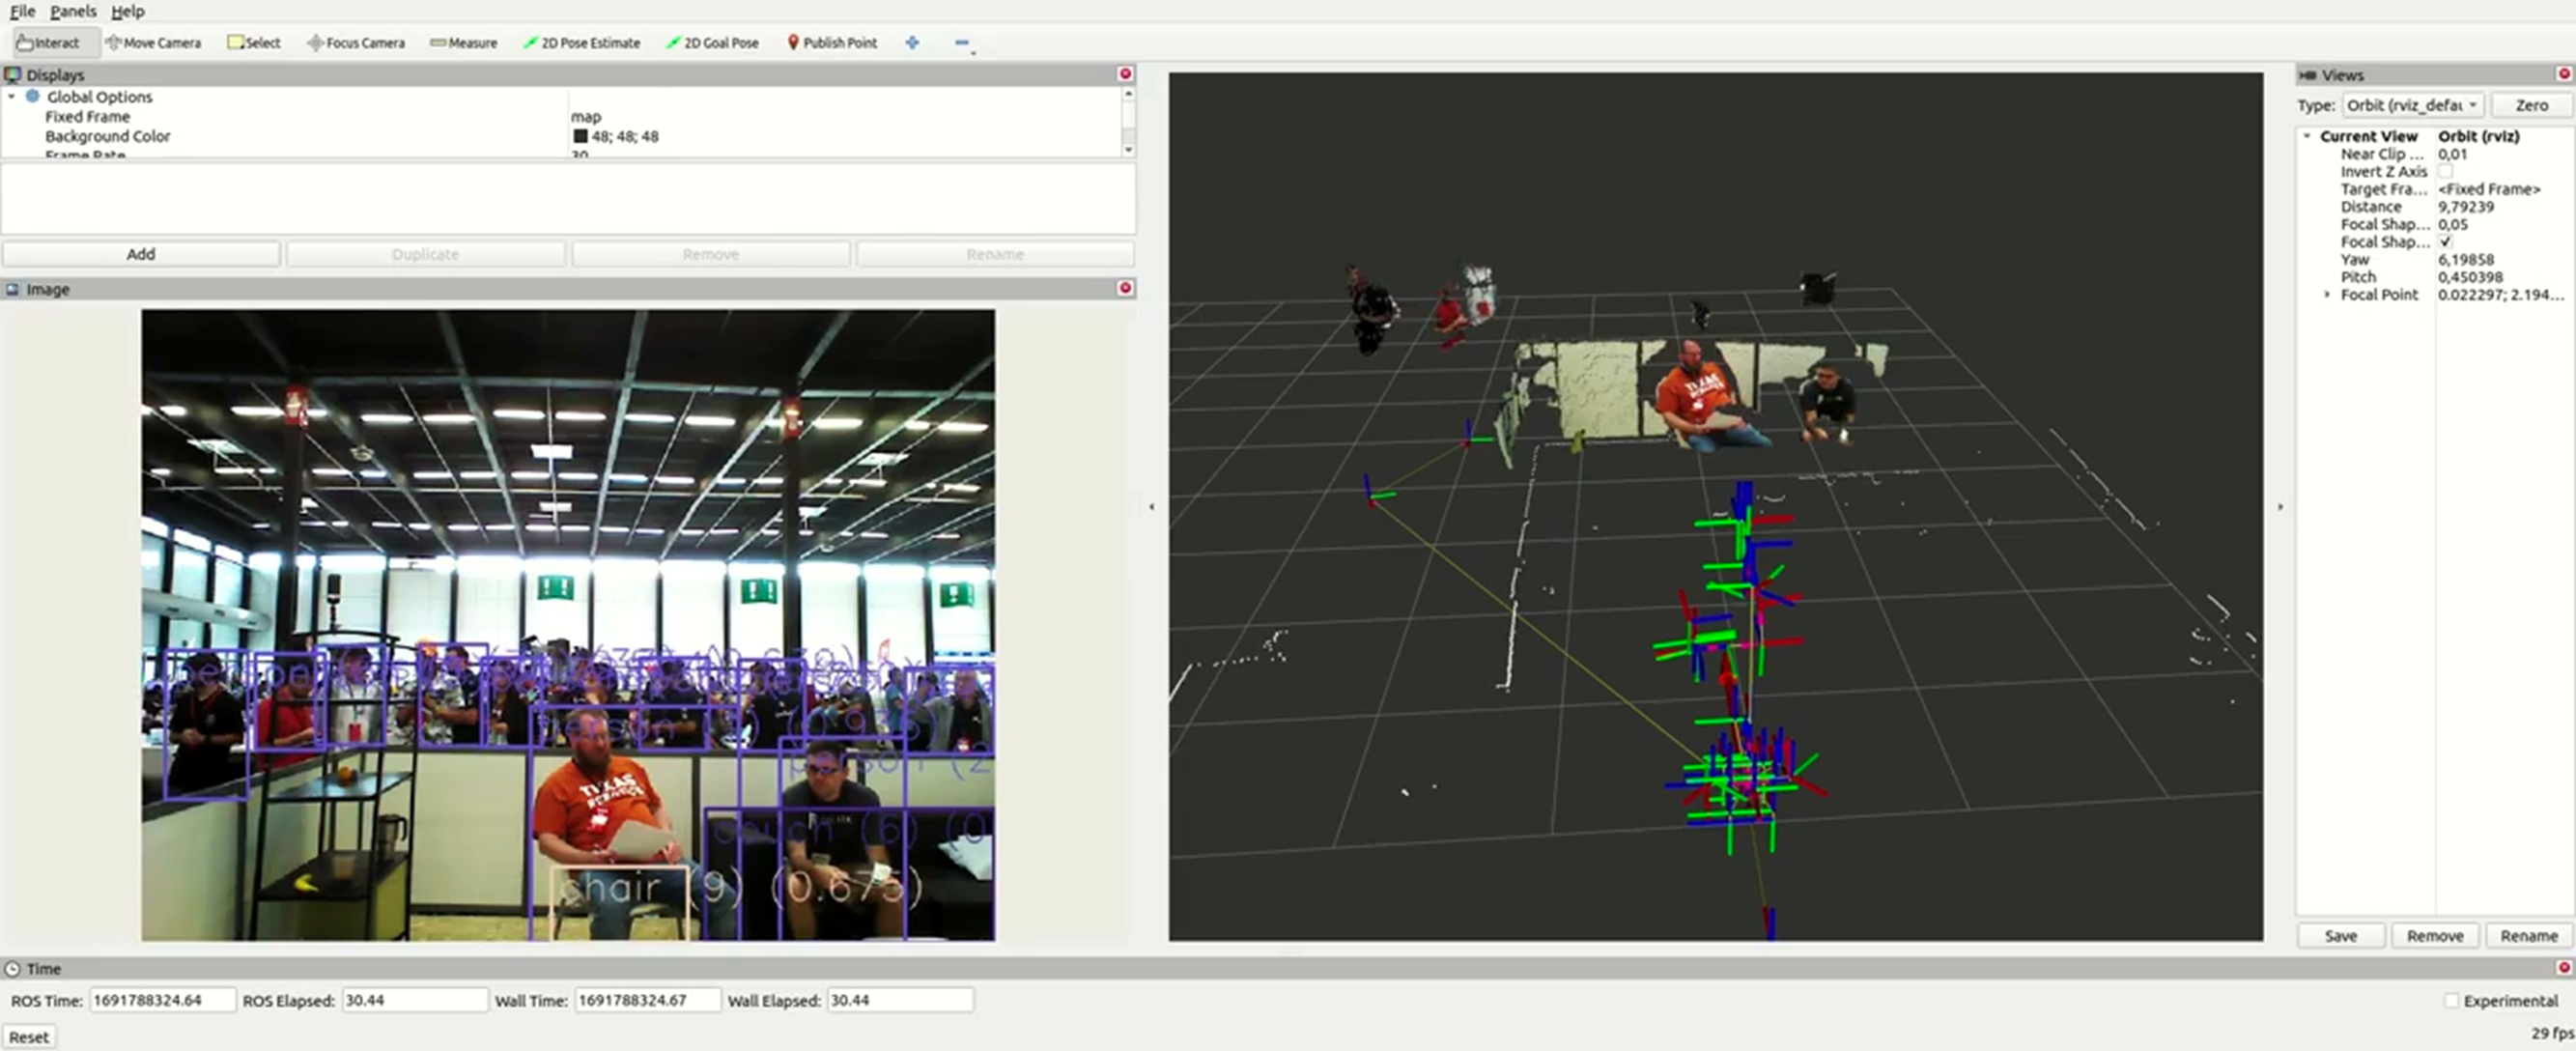
\includegraphics[width=0.95\linewidth,height=0.58\textheight,keepaspectratio]{images/tema_3/4_2_s05_deteccion-de-objetos-segmentacion-de-instancias_img01.png}
    \end{column}
  \end{columns}
\end{frame}

\begin{frame}{Detección de objetos: humanos}
  \small
  \begin{columns}[T,onlytextwidth]
    \begin{column}{0.58\textwidth}
      \begin{itemize}
        \item \$ ros2 launch yolov8\_bringup yolov8.launch.py model:=src/sensors/models/yolov8m-pose.pt image\_reliability:=1 input\_image\_topic:=/camera/color/image\_raw
      \end{itemize}
      \begin{itemize}
        \item Se parte de un conjunto de datos (dataset):
        \item Conjunto de entrenamiento
        \item Conjunto de validación
      \end{itemize}
    \end{column}
    \begin{column}{0.42\textwidth}
    \centering
    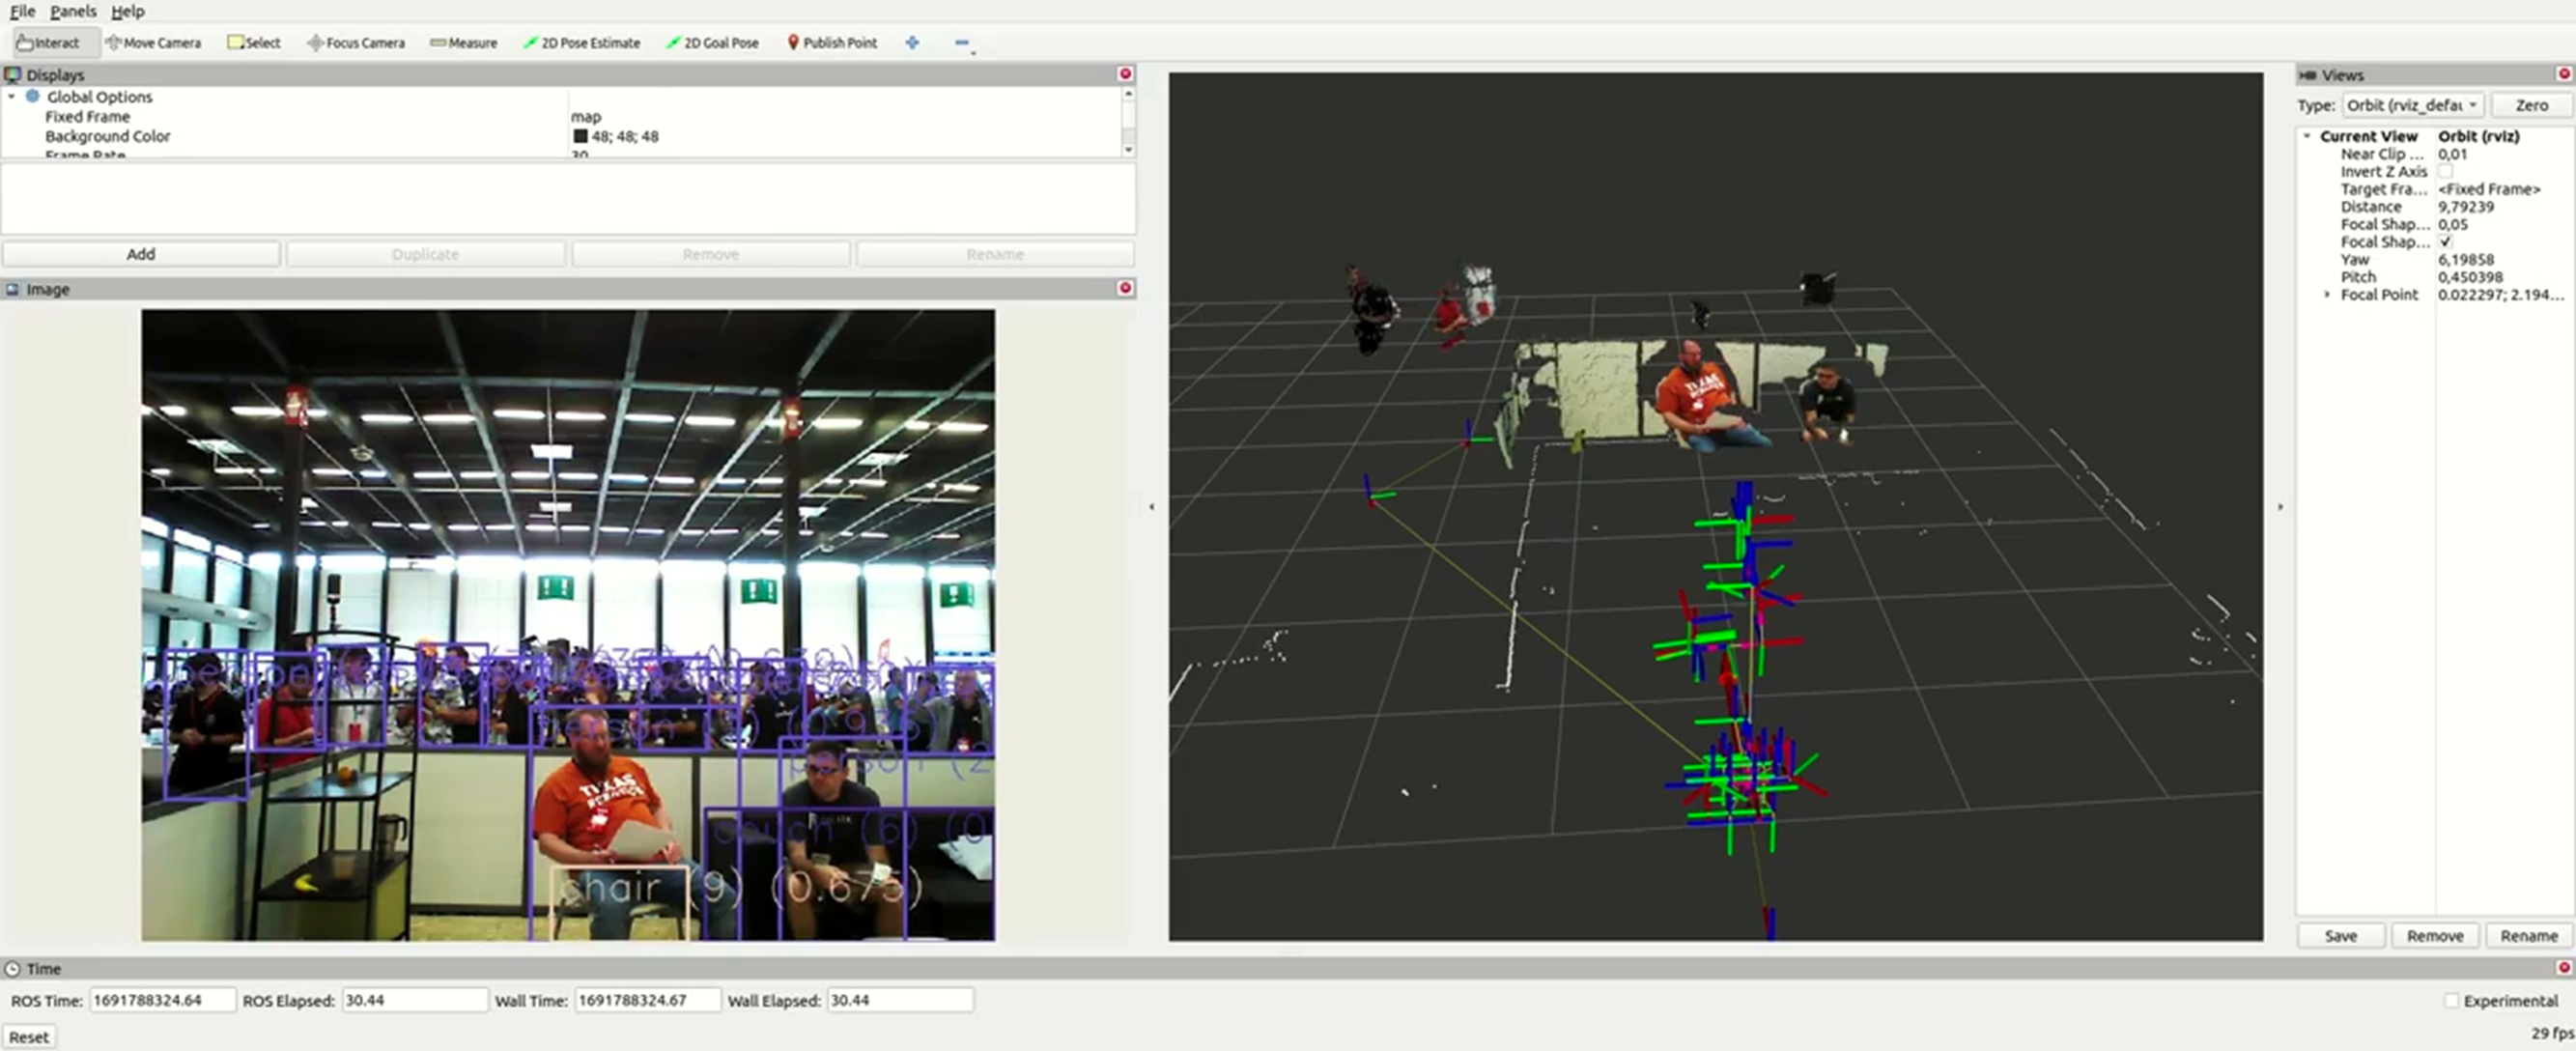
\includegraphics[width=0.95\linewidth,height=0.58\textheight,keepaspectratio]{images/tema_3/4_2_s06_deteccion-de-objetos-humanos_img01.png}
    \end{column}
  \end{columns}
\end{frame}

\begin{frame}{Detección de objetos: segmentación de}
  \small
  \begin{columns}[T,onlytextwidth]
    \begin{column}{0.58\textwidth}
      \begin{itemize}
        \item instancias
        \item \$ ros2 launch yolov8\_bringup yolov8\_3d.launch.py model:=src/sensors/models/yolov8m-seg.pt image\_reliability:=2 input\_image\_topic:=/camera/color/image\_raw input\_depth\_topic:=/camera/depth/image\_raw target\_frame:=camera\_color\_optical\_frame
      \end{itemize}
      \begin{itemize}
        \item Se parte de un conjunto de datos (dataset):
        \item Conjunto de entrenamiento
        \item Conjunto de validación
      \end{itemize}
    \end{column}
    \begin{column}{0.42\textwidth}
    \centering
    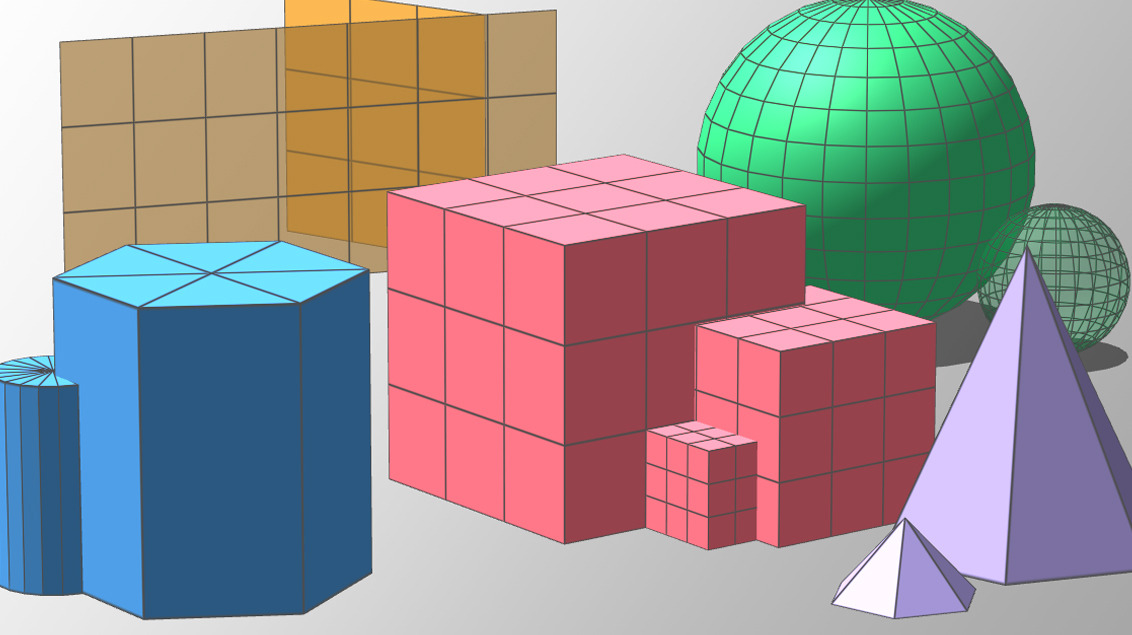
\includegraphics[width=0.95\linewidth,height=0.58\textheight,keepaspectratio]{images/tema_3/4_2_s07_deteccion-de-objetos-segmentacion-de-instancias_img01.png}
    \end{column}
  \end{columns}
\end{frame}

\section{Interfaces YOLOv8}

\begin{frame}{Interfaces de detección (YOLOv8)}
  \small
  \begin{itemize}
    \item El resultado útil no es solo una imagen anotada, sino una estructura de detecciones.
    \item En ROS 2 se recomienda publicar con \textbf{vision\_msgs}:
    \begin{itemize}
      \item \texttt{Detection2DArray} para cajas en imagen,
      \item \texttt{Detection3DArray} para detecciones en 3D.
    \end{itemize}
    \item Cada detección incluye clase, confianza y localización.
    \item Esto desacopla percepción y decisión: navegación o interacción consumen detecciones, no píxeles crudos.
  \end{itemize}
\end{frame}

\section{Percepción 3D}

\begin{frame}{Percepción 3D y nubes de puntos}
  \small
  \begin{itemize}
    \item Sensores RGBD, ToF y LiDAR 3D permiten estimar geometría del entorno.
    \item Formato estándar en ROS 2: \textbf{sensor\_msgs/msg/PointCloud2}.
    \item La nube de puntos se usa para:
    \begin{itemize}
      \item segmentación de objetos,
      \item detección de planos y obstáculos,
      \item localización y mapeado.
    \end{itemize}
    \item Requiere filtrado y gestión eficiente por el gran volumen de datos.
  \end{itemize}
\end{frame}

\section{Ejemplo (sensors/camera)}

\begin{frame}{Detección de objetos: segmentación de}
  \small
  \begin{columns}[T,onlytextwidth]
    \begin{column}{0.58\textwidth}
      \begin{itemize}
        \item instancias
      \end{itemize}
      \begin{itemize}
        \item Pipeline de percepción:
        \item 2 posibles ‘fuentes’ de percepción
        \item Utilización de vision\_msgs
        \item Deseable $\rightarrow$ nodo que publicara TFs con las detecciones
      \end{itemize}
    \end{column}
    \begin{column}{0.42\textwidth}
    \centering
    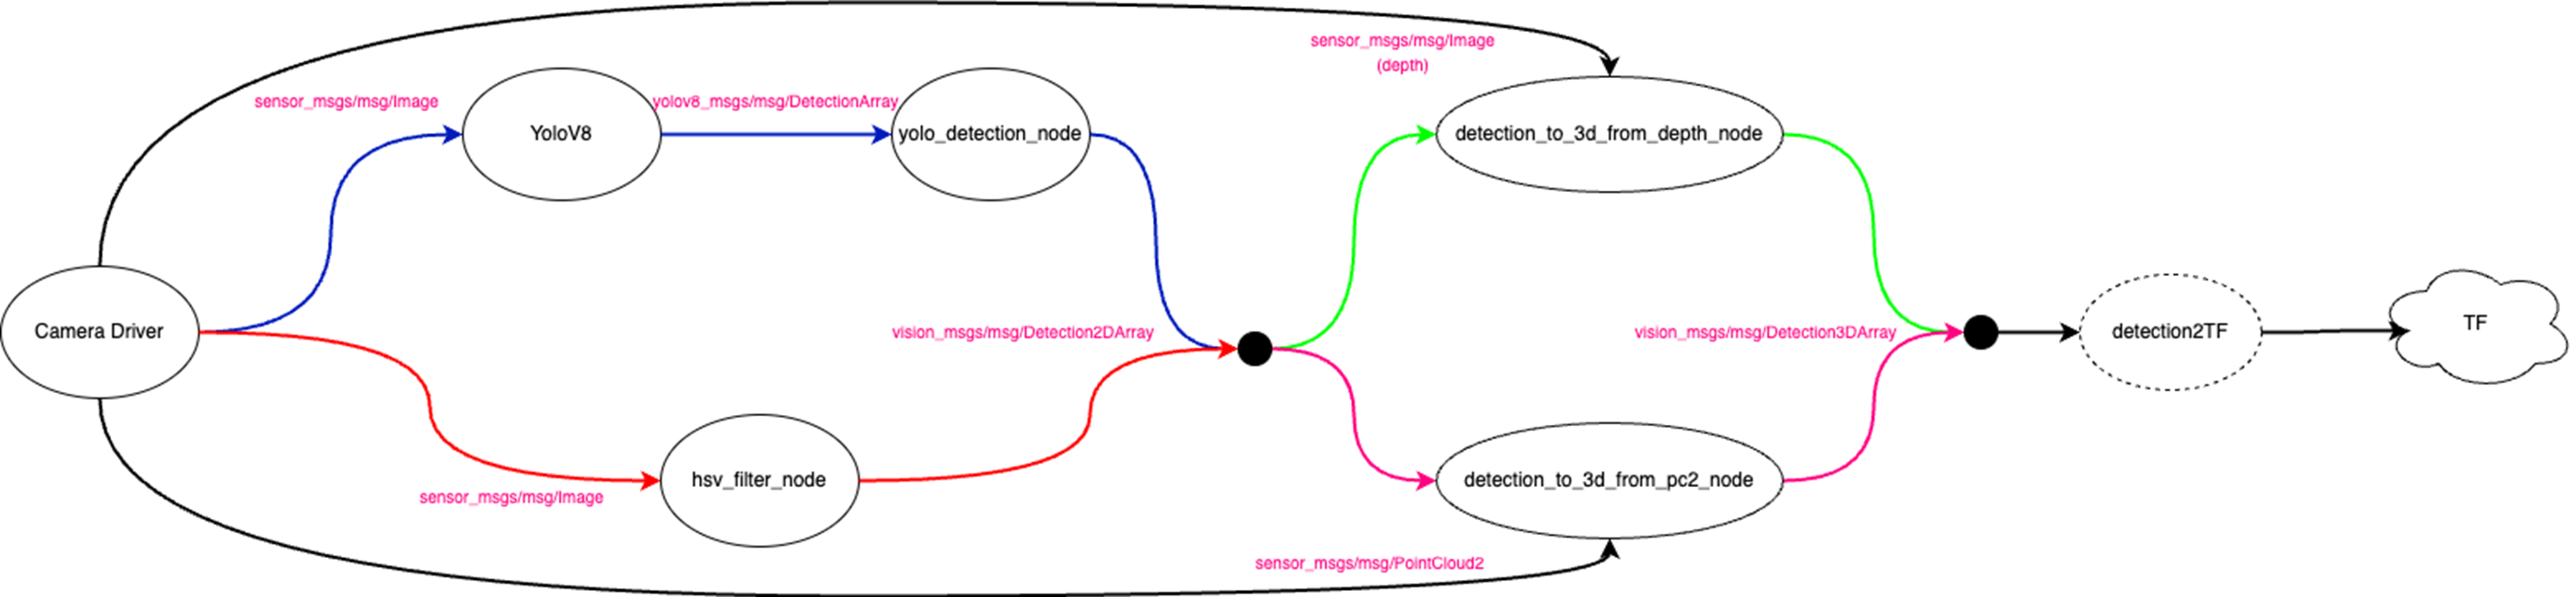
\includegraphics[width=0.95\linewidth,height=0.58\textheight,keepaspectratio]{images/tema_3/4_2_s11_deteccion-de-objetos-segmentacion-de-instancias_img01.png}
    \end{column}
  \end{columns}
\end{frame}

\begin{frame}{Detección de objetos: segmentación de}
  \small
  \begin{columns}[T,onlytextwidth]
    \begin{column}{0.58\textwidth}
      \begin{itemize}
        \item instancias
      \end{itemize}
      \begin{itemize}
        \item Pipeline de percepción:
        \item 2 posibles ‘fuentes’ de percepción
        \item Utilización de vision\_msgs
        \item Deseable $\rightarrow$ nodo que publicara TFs con las detecciones
      \end{itemize}
    \end{column}
    \begin{column}{0.42\textwidth}
    \centering
    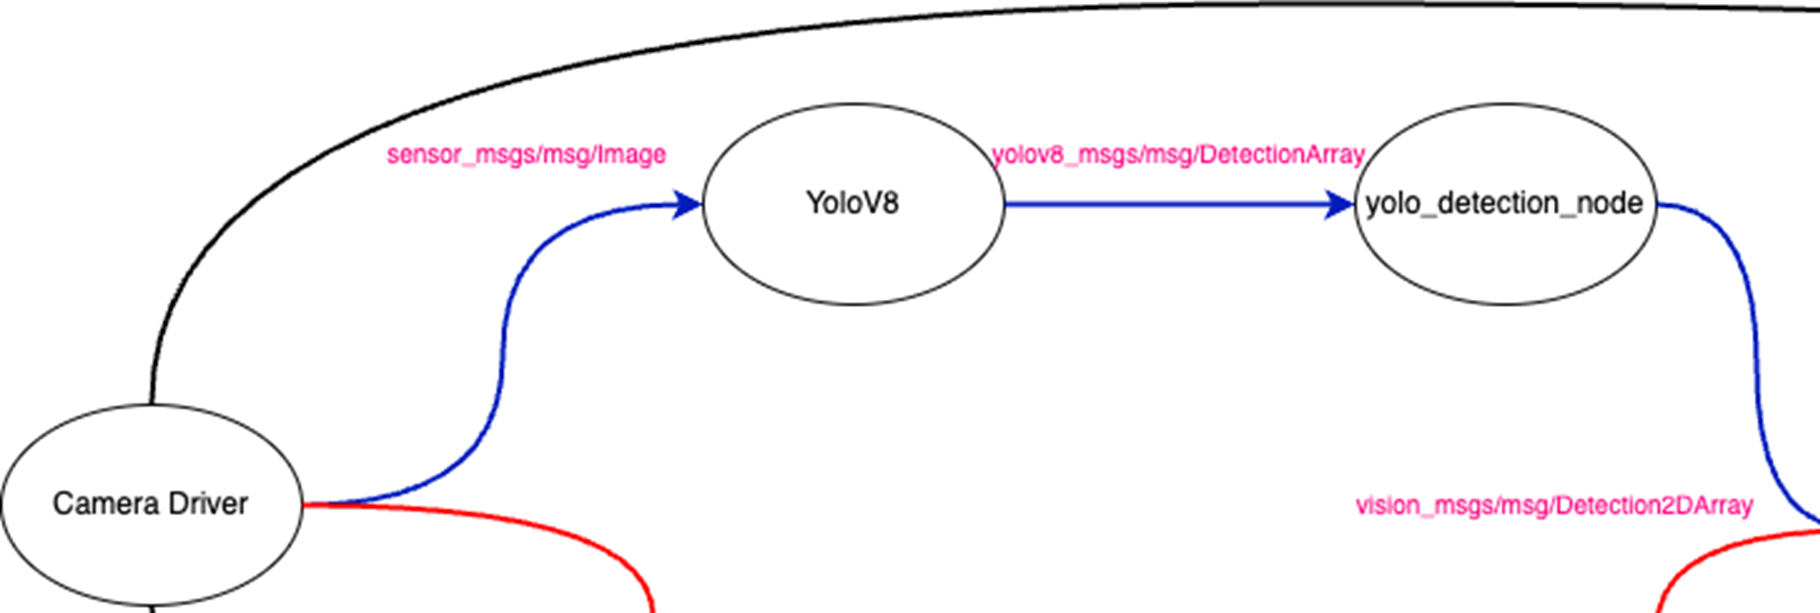
\includegraphics[width=0.95\linewidth,height=0.58\textheight,keepaspectratio]{images/tema_3/4_2_s12_deteccion-de-objetos-segmentacion-de-instancias_img01.png}
    \end{column}
  \end{columns}
\end{frame}

\begin{frame}{Detección de objetos: segmentación de}
  \small
  \begin{columns}[T,onlytextwidth]
    \begin{column}{0.58\textwidth}
      \begin{itemize}
        \item instancias
      \end{itemize}
      \begin{itemize}
        \item Pipeline de percepción:
        \item 2 posibles ‘fuentes’ de percepción
        \item Utilización de vision\_msgs
        \item Deseable $\rightarrow$ nodo que publicara TFs con las detecciones
      \end{itemize}
    \end{column}
    \begin{column}{0.42\textwidth}
    \centering
    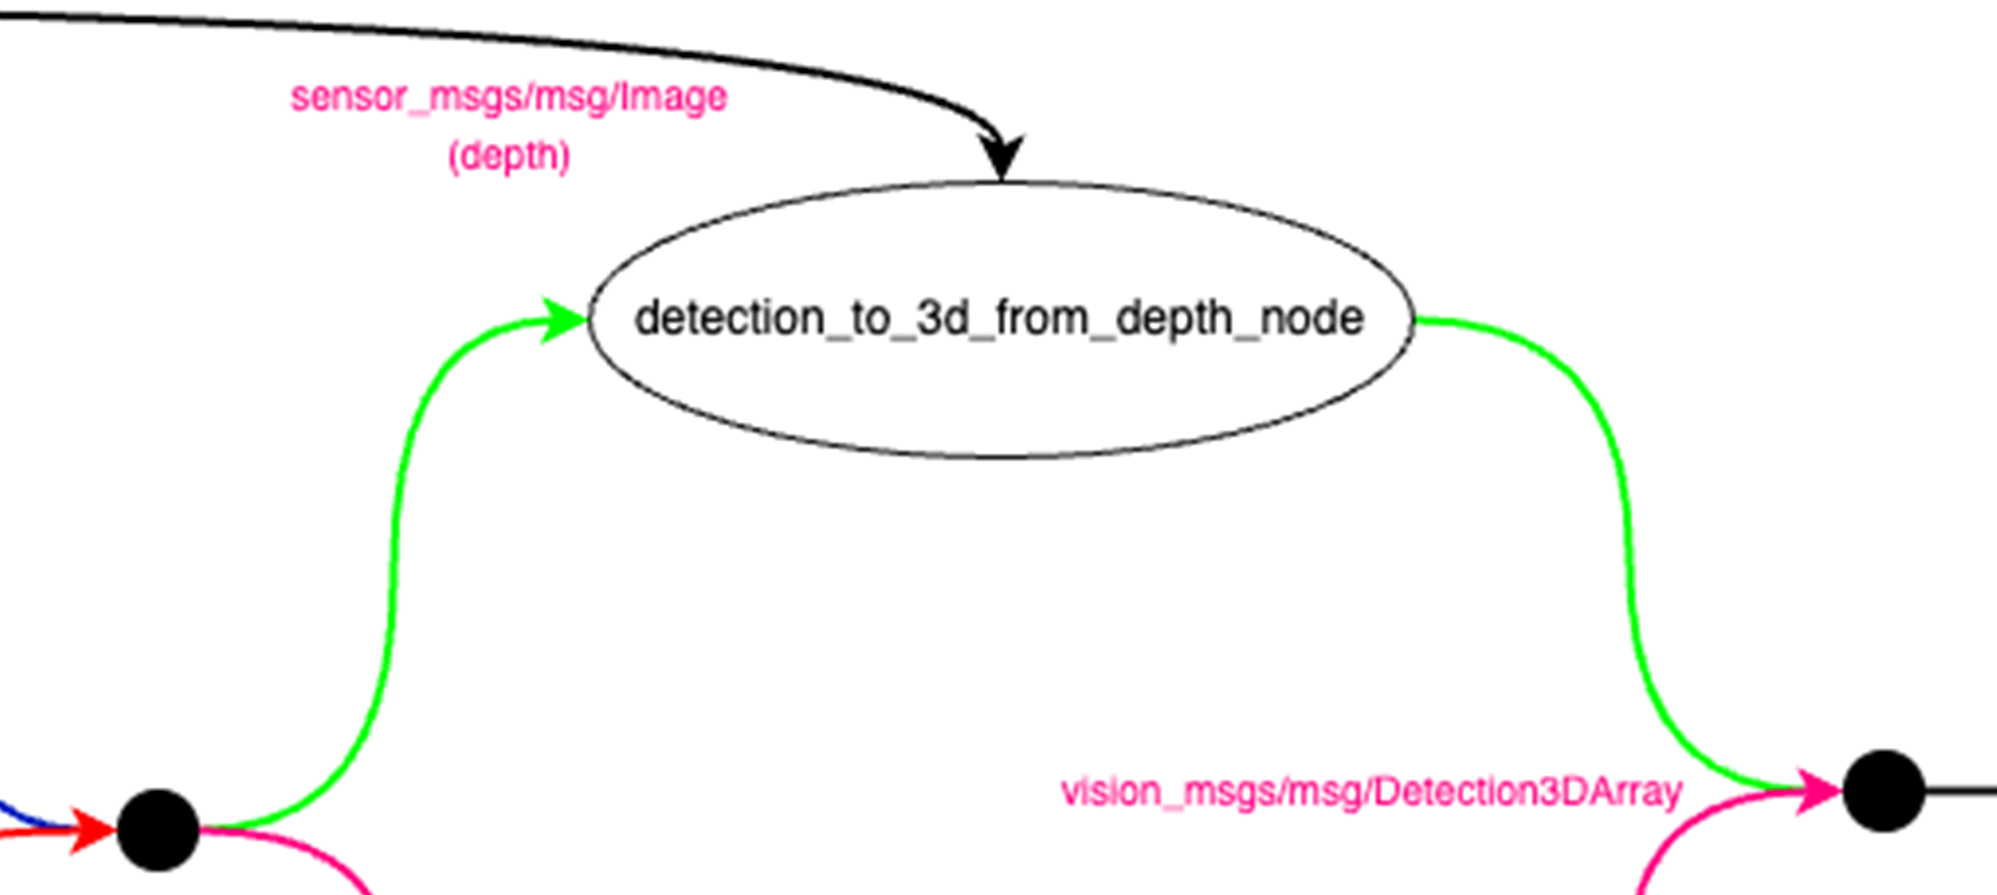
\includegraphics[width=0.95\linewidth,height=0.58\textheight,keepaspectratio]{images/tema_3/4_2_s13_deteccion-de-objetos-segmentacion-de-instancias_img01.png}
    \end{column}
  \end{columns}
\end{frame}

\begin{frame}{Detección de objetos: segmentación de}
  \small
  \begin{columns}[T,onlytextwidth]
    \begin{column}{0.58\textwidth}
      \begin{itemize}
        \item instancias
      \end{itemize}
      \begin{itemize}
        \item Pipeline de percepción:
        \item 2 posibles ‘fuentes’ de percepción
        \item Utilización de vision\_msgs
        \item Deseable $\rightarrow$ nodo que publicara TFs con las detecciones
      \end{itemize}
    \end{column}
    \begin{column}{0.42\textwidth}
    \centering
    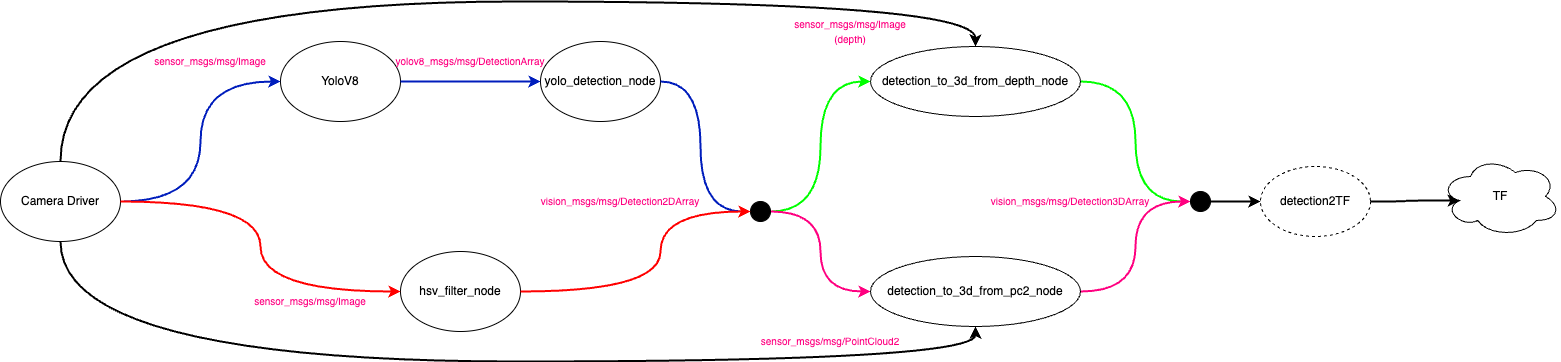
\includegraphics[width=0.95\linewidth,height=0.58\textheight,keepaspectratio]{images/tema_3/4_2_s14_deteccion-de-objetos-segmentacion-de-instancias_img01.png}
    \end{column}
  \end{columns}
\end{frame}

\section{PID}

\section{Ejemplo (tf\_seeker)}

\section{Librería PID}


\begin{frame}{Percepción}
  \small
  \begin{itemize}
    \item deep learning y 3D
  \end{itemize}
\end{frame}

\end{document}
